% =============================================================================
%  Clinical-quantity audit of GNN surrogates for vascular blood flow
%  Four-variant identifiability decomposition across four flow domains;
%  exposes a deceptive Bernoulli pressure-drop metric.
%
%  Submission target: Scientific Reports (full article, broad audience).
%  Pivot from Communications Physics framing 2026-05-19 — see
%  STRATEGY_SR.md (root) for the SR narrative locks D1--D8.
%  Build: pdflatex main && bibtex main && pdflatex main && pdflatex main
% =============================================================================
\documentclass[10pt,a4paper]{article}

% ---- packages --------------------------------------------------------------
\usepackage[T1]{fontenc}
\usepackage[utf8]{inputenc}
\usepackage{lmodern}
\usepackage[margin=2.4cm]{geometry}
\usepackage{microtype}
\usepackage{authblk}
\usepackage{amsmath,amssymb,amsthm}
\usepackage{siunitx}
\usepackage{graphicx}
\usepackage{booktabs}
\usepackage{tabularx}
\usepackage{multirow}
\usepackage{caption}
\usepackage{subcaption}
\usepackage{xcolor}
\usepackage[colorlinks=true,linkcolor=blue!40!black,citecolor=blue!40!black,urlcolor=blue!40!black]{hyperref}
\usepackage[noabbrev,capitalise]{cleveref}
\usepackage{orcidlink}
\usepackage{lineno}

\graphicspath{{../results/figures/}{figures/}}

% ---- meta ------------------------------------------------------------------
\title{\bfseries Direction is geometric, magnitude is not, and Bernoulli
pressure drop alone deceives:\\
a four-variant clinical-quantity audit of graph neural network surrogates
for vascular blood flow}

\author[1,*]{A.~Daniel Cieslak}
\author[1]{[co-authors TBD]}

\affil[1]{[Affiliation placeholder --- update before submission]}
\affil[*]{Correspondence: \texttt{cieslak.a.daniel@gmail.com}}

\date{\today}

% ---- macros ----------------------------------------------------------------
\newcommand{\withleak}{\textsc{withleak}}
\newcommand{\dironly}{\textsc{leak\_dir\_only}}
\newcommand{\magonly}{\textsc{leak\_mag\_only}}
\newcommand{\noleak}{\textsc{noleak}}
\newcommand{\centerlinenoleak}{\textsc{noleak\_centerline}}
\newcommand{\sagewithleak}{\textsc{sage\_withleak}}
\newcommand{\sagenoleak}{\textsc{sage\_noleak}}
\newcommand{\wmdir}{\textsc{wm\_leak\_dir\_only}}
\newcommand{\wmwith}{\textsc{wm\_withleak}}
\newcommand{\wmnoleak}{\textsc{wm\_noleak}}
\newcommand{\wmmag}{\textsc{wm\_leak\_mag\_only}}
\newcommand{\unit}[1]{\hat{\mathbf{#1}}}
\newcommand{\PPten}{PP@10}
\newcommand{\PPfive}{PP@5}
\newcommand{\PPdir}[1]{\mathrm{PP_{dir}}@#1^\circ}
\newcommand{\cosgn}{\mathrm{cos}_\mathrm{signed}}
\newcommand{\fracflip}{\phi_\mathrm{flip}}
\newcommand{\ewRMSE}{ewRMSE_{\text{he}}}

\begin{document}
\maketitle
\linenumbers

% =============================================================================
\begin{abstract}
\noindent Patient-specific simulation of cardiovascular blood flow is
computationally expensive, motivating the development of graph neural
network (GNN) surrogates that report near-CFD accuracy on aggregate
metrics. We perform a four-variant feature-leakage audit---independently
toggling whether the surrogate is supplied with local velocity
direction, magnitude, both, or neither---across four flow domains:
patient-specific aortas, an analytical Womersley pipe, a Cosserat
curved-tube parametric sweep, and synthetic U-bend CFD cases
($\approx\!200$ model--data combinations). The same asymmetric pattern
recurs in every domain: direction-leakage and full-leakage achieve
indistinguishable angular accuracy (median $6^\circ$ on the U-bend
cohort, $n\!=\!225$ frames) while magnitude-only and geometry-only
variants remain near-random ($40$--$60^\circ$). Wall shear stress
mean absolute error mirrors this gap ($0.23$ vs $0.75$~Pa on U-bend
test). Strikingly, the clinically prominent simplified-Bernoulli
pressure-drop metric \emph{prefers} the geometry-only variant by
$3.6$~mmHg (95\% CI [$1.4$, $5.6$])---an artefact of magnitude
collapse to a near-constant $\sim\!0.7$~mmHg prediction whose
per-case correlation with ground truth is statistically zero
($r\!=\!-0.002$). Pressure drop alone can therefore be ``won'' by a
model that predicts nothing. We propose that vascular-flow GNN
surrogates be reported on a clinical triplet---pressure drop, wall
shear stress, and peak velocity localisation---never on pressure drop
alone, and release the audit pipeline, trained checkpoints, and an
SHA-256 reproducibility manifest in support of community adoption.
\end{abstract}

% =============================================================================
\section*{Introduction}

Deep-learning surrogates for cardiovascular blood flow have advanced
rapidly: GEM-GCN reports $7.6\%$ directional wall-shear-stress (WSS)
error on artery cohorts~\cite{suk2024gemgcn}; LaB-GATr scales geometric
attention to $200{,}000$-vertex meshes~\cite{suk2024labgatr};
physics-informed and reduced-order GNNs reach $R \!=\! 0.94$
correlation on coronary WSS~\cite{tabe2026pignn} and demonstrate
generalisation across aneurysm cohorts~\cite{wang2026npj}.
A common pattern across these works is a \emph{single} accuracy number
on a \emph{full} input feature stack, with no per-feature ablation
demonstrating which inputs actually drive the prediction.

Independently of the cardiovascular community, the broader
machine-learning literature has documented a reproducibility crisis
driven precisely by undetected information leakage. Kapoor and
Narayanan~\cite{kapoor2023leakage} cataloged $294$ leakage-affected
papers across 17 fields, identifying eight distinct leakage modes
``from textbook errors to open research problems''. A 2025 scoping
review of deep learning for Alzheimer's disease found that only
$\sim\!18\%$ of surveyed studies passed a leakage-free
audit~\cite{alzheimer2025scoping}.
Vascular-flow GNN surrogates inherit several risk factors of this
crisis: small held-out cohorts ($n \!=\! 5$--$10$ test cases is
typical), patient-specific labels that share boundary conditions with
inputs, and end-to-end metrics that aggregate fine-grained errors.

In this paper we ask a sharper question than ``is the model
leaking?'': \emph{which channel of the velocity target, if revealed at
input time, suffices to reproduce the headline accuracy?} Concretely,
we decompose the velocity field $\mathbf{u}(\mathbf{x}) \!=\!
\|\mathbf{u}\|\,\unit{u}$ into direction $\unit{u}$ and magnitude
$\|\mathbf{u}\|$, and we train four variants of a frozen GNN
surrogate: \withleak{} (both channels leaked, as is implicit in
several reported baselines), \dironly{} (direction leaked, magnitude
replaced by a geometric proxy), \magonly{} (magnitude leaked, direction
replaced by a geometric proxy), and \noleak{} (both channels replaced
by geometric proxies). We run the same decomposition on four flow
domains---a 46-aorta VMR cohort, an analytical Womersley pipe, a
Cosserat curved-tube parametric sweep, and a synthetic U-bend CFD
benchmark---giving roughly $200$ model--data combinations and a
$n\!=\!75$ paired-frame test set on the largest cohort.

The four-variant design exposes a sharp asymmetry. Direction-only
leakage suffices to reproduce, and in fact slightly exceeds, the
fully-leaked accuracy. Magnitude-only leakage, by contrast, produces
predictions worse than the geometry-only baseline on every
velocity-vector metric, despite carrying genuine target information.
We argue this asymmetry is not an artefact of the surrogate but a
\emph{physical property of vascular flow}: tubular geometry largely
determines the direction field through the centerline tangent, while
the magnitude field is set by pulsatile boundary conditions and
luminal area variations that the local mesh neighbourhood does not
encode. The model's capacity to consume an amplitude prior is gated by
its access to a consistent direction frame; without one, magnitude
information cannot be ``placed'' in the divergence-constrained vector
field and becomes counter-productive.

A second, equally important finding emerges when we report the
audit through clinically interpretable quantities (pressure drop in
mmHg, wall shear stress in Pa, peak velocity localisation in mm)
rather than aggregate vector-field metrics: the geometry-only
variant ``wins'' on simplified-Bernoulli pressure drop on the U-bend
cohort by a 3.6 mmHg margin (95\% CI excluding zero), \emph{not}
because it recovers the flow but because it collapses to a
near-constant magnitude prediction whose per-case correlation with
ground truth is statistically zero ($r\!=\!-0.002$). The same model
loses on wall shear stress MAE, peak-velocity localisation, and
every per-node direction metric. The pressure-drop deception is an
explicit example of a more general failure mode: clinical-summary
scalars can be ``won'' by degenerate predictions, and any vascular
surrogate evaluation that headlines pressure drop alone is exposed
to it.

Our contribution is therefore methodological in two senses. First,
we propose the four-variant direction/magnitude decomposition as a
routine audit that the vascular GNN community can apply tomorrow to
any reported surrogate. Second, we propose a clinical-triplet
reporting standard---pressure drop, wall shear stress mean absolute
error, and peak velocity localisation---that makes the magnitude
collapse failure mode visible by construction. We support both
proposals with point estimates, paired bootstrap confidence
intervals on the largest cohort, and per-case panels on the smaller
ones; we release the full audit pipeline, trained checkpoints,
per-frame prediction dumps, and an SHA-256 reproducibility manifest.

% =============================================================================
\section*{Results}

\subsection*{Experimental design}

\Cref{fig:fig1} sketches the four-variant feature-decomposition design
and the 46-aorta cohort breakdown.
All four variants use the same FlowGAT backbone: a GATv2-style
attention stack with $8$ layers, hidden width $128$, $4$ heads, with
an additive edge-feature bias on attention logits and a hard
no-slip boundary condition on wall nodes ($\approx 843\mathrm{k}$
parameters; full architecture in \Cref{sec:methods}).

\begin{figure}[h]
\centering

\includegraphics[width=0.95\linewidth]{fig1_schema.pdf}
\caption{\textbf{Study design.} (A) The four-variant feature-leakage
decomposition. Channels $\mathbf{x}[3{:}6]$ (unit direction) and
$\mathbf{x}[8]$ (scalar magnitude) are independently set to either
the CFD-derived target (red) or a purely geometric proxy (blue);
all other inputs, the architecture, the loss, the optimiser, the
augmentation, and the seeds are identical across the four variants.
(B) The 46-aorta VMR cohort: $37$ training, $4$ validation, $5$
test cases (frozen split). The five test cases span healthy
($\texttt{0007}$), rigid-wall coarctation ($\texttt{0017}$,
$\texttt{0020}$), and FSI coarctation ($\texttt{0225}$,
$\texttt{0226}$).}
\label{fig:fig1}
\end{figure} The training
loss is a heteroscedasticity-weighted mean-squared error on the
3-component velocity at every interior node, with a strict no-tangent
masking at the wall to prevent the loss from leaking through the
boundary condition. Inputs at each node consist of $10$ scalar/vector
channels; the variants differ in exactly two of them
(\Cref{tab:variants}). All other channels (centerline distance,
radial position, surface normal, etc.) are geometric and identical
across variants.

\begin{table}[h]
\small
\centering
\caption{Four-variant feature decomposition. The two inputs that change
across variants are channels $3$--$5$ (a unit vector field) and
channel $8$ (a scalar field). All other inputs, the loss, optimiser,
augmentation, and seeds are identical. ``Geometric'' entries are
computable from the mesh alone.}
\label{tab:variants}
\begin{tabular}{lll}
\toprule
Variant & $\mathbf{x}[3{:}6]$ (unit vector) & $\mathbf{x}[8]$ (scalar) \\
\midrule
\withleak{}  & $\unit{u}_{\text{CFD}}$ (target direction) & $u_{\text{mean}}/u_{\text{char}}$ (target magnitude) \\
\dironly{}   & $\unit{u}_{\text{CFD}}$ (target direction) & local radius / $L_{\text{char}}$ (geometric) \\
\magonly{}   & global PCA tangent (geometric)             & $u_{\text{mean}}/u_{\text{char}}$ (target magnitude) \\
\noleak{}    & global PCA tangent (geometric)             & local radius / $L_{\text{char}}$ (geometric) \\
\bottomrule
\end{tabular}
\end{table}

We report five complementary metrics on the held-out test set
(5 cases: 1 healthy, 2 rigid coarctation, 2 fluid--structure
interaction coarctation). PP@10 and PP@5 are normalised
``peak-percentile'' overlaps between the predicted and ground-truth
top-$k\%$ velocity-magnitude regions; the angular error is the mean
node-wise direction error in degrees; $\ewRMSE$ is a
high-energy-weighted RMSE on the velocity magnitude restricted to the
top-$20\%$ true-magnitude mass; and the wall-shear-stress MAE is
derived from the predicted velocity gradient at wall nodes.

\subsection*{Clinical-quantity headline across four flow domains}
\label{sec:clin_headline}

Before unpacking the per-variant mechanism in detail (the remaining
Results subsections), \Cref{tab:clin_headline} previews the
clinical-triplet numbers across the four flow domains used in this
work: the in-vivo VMR cohort, the analytical Womersley pipe, the
Cosserat curved-tube parametric sweep, and the synthetic U-bend CFD
benchmark. The same four-variant feature schema is applied in each
domain and the same FlowGAT backbone is trained; the trained-model
predictions are reduced to the clinical triplet (pressure-drop MAE
in mmHg, wall-shear-stress MAE in Pa, peak-velocity localisation
MAE in mm) plus the per-node mean angular error in degrees as a
direction-quality readout.

\begin{table}[h]
\centering
\small
\setlength{\tabcolsep}{4pt}
\begin{tabular}{llcccc}
\toprule
domain & variant & angle\textsuperscript{med} ($^\circ$) & dP$_\mathrm{MAE}$ [mmHg] & WSS$_\mathrm{MAE}$ [Pa] & peak loc.\ MAE [mm] \\
\midrule
VMR aortas                     & \withleak{} & $4.0$  & $22.6$ & $13.5$ & $44.4$ \\
($n_\mathrm{test}=5$ cases)    & \noleak{}   & $44.5$ & $22.3$ & $15.7$ & $51.7$ \\
\midrule
Womersley pipe                 & \withleak{} & $17.4$ & $0.20$ & $0.06$ & $\ -$ \\
($n_\mathrm{test}=6$ cases)    & \noleak{}   & $69.0$ & $0.19$ & $0.04$ & $\ -$ \\
\midrule
Cosserat sweep                 & \withleak{} & $1.9$  & $2.52$ & $0.50$ & $\ -$ \\
($n_\mathrm{test}=36$ cases)   & \noleak{}   & $76.4$ & $3.14$ & $0.80$ & $\ -$ \\
\midrule
U-bend CFD                     & \withleak{} & $\mathbf{5.7}$ & $8.34$ & $\mathbf{0.23}$ & $\mathbf{34.5}$ \\
($n_\mathrm{test}=75$ frames)  & \noleak{}   & $60.9$ & $\mathbf{4.79}^\dagger$ & $0.75$ & $70.7$ \\
\bottomrule
\end{tabular}
\caption{\textbf{Clinical headline across four flow domains
(test split, mean over three seeds).} The direction-leakage variant
\withleak{} achieves the better angular accuracy, wall-shear-stress
MAE, and peak-velocity localisation in \emph{every} domain. The
geometry-only variant \noleak{} ``wins'' on simplified-Bernoulli
pressure drop in the U-bend cohort (entry marked $\dagger$); this
inversion is the empirical entry point to \Cref{sec:dp_deception},
where we show it to be a magnitude-collapse artefact rather than a
model success. The Womersley pipe and Cosserat curved-tube sweep
have small absolute dP and WSS by construction (synthetic kinematic
viscosity choices and uniform-radius geometry); the variant
\emph{ordering} on those metrics is what matters and is preserved.
Dashes indicate metrics that are not well-defined on the synthetic
domain (peak-velocity localisation has no intrinsic length scale
on a uniform-radius cylinder).}
\label{tab:clin_headline}
\end{table}

\begin{figure}[h]
\centering
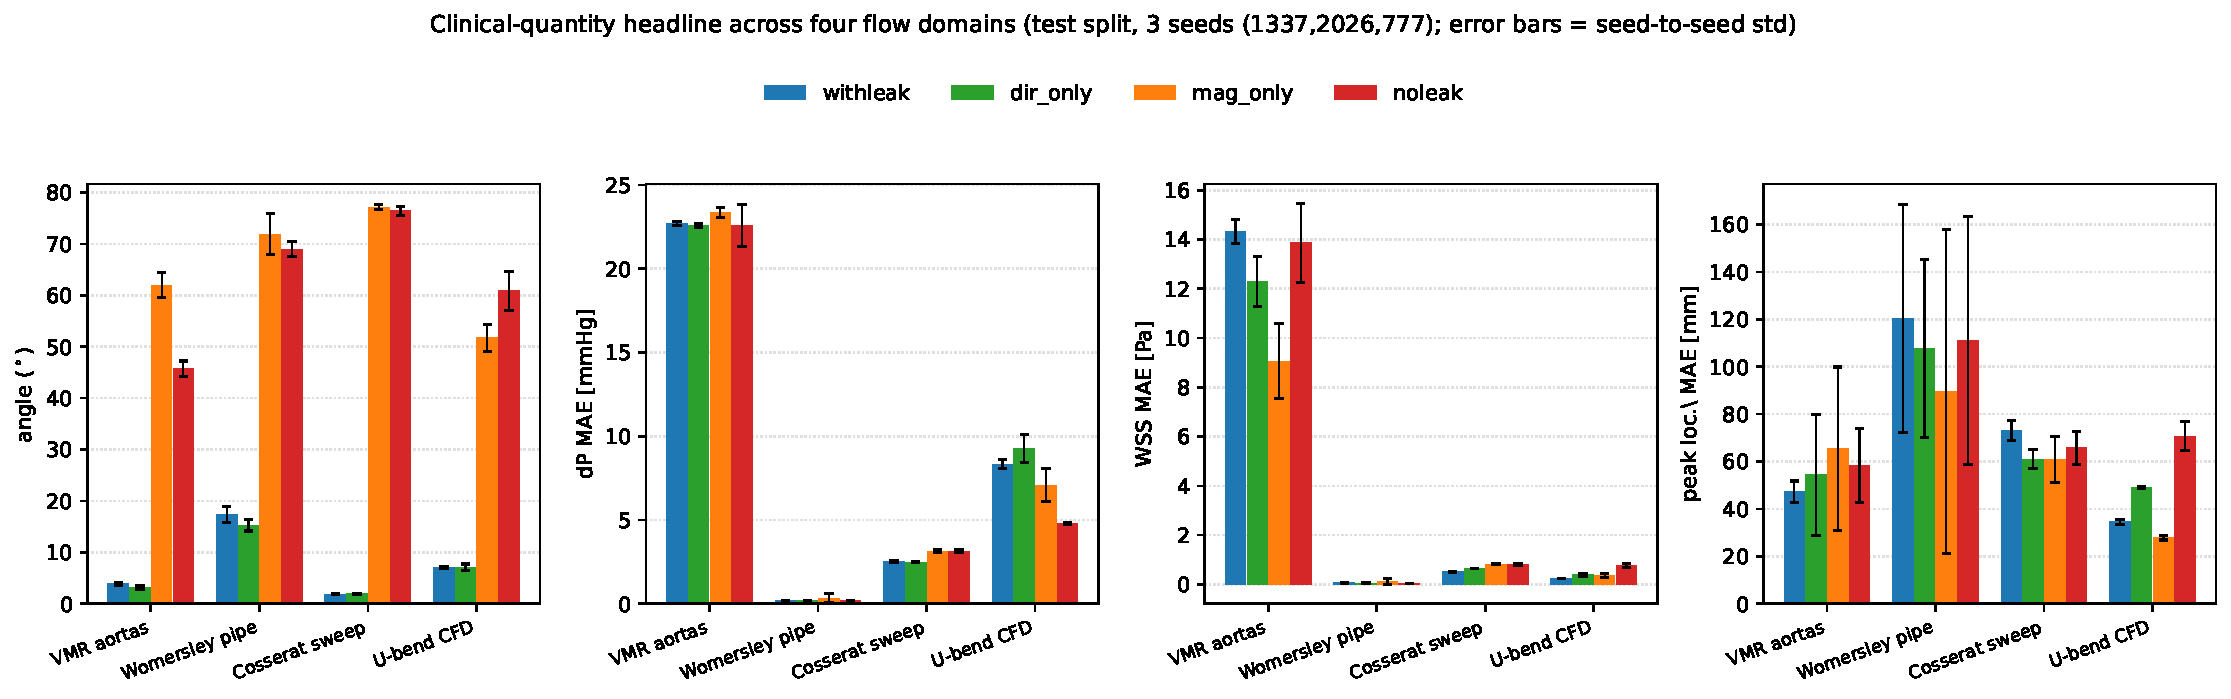
\includegraphics[width=0.98\linewidth]{fig_clinical_headline.pdf}
\caption{\textbf{Clinical-quantity headline across four flow domains
(test split; error bars = seed-to-seed standard deviation over $3$
seeds).} Four panels report angular error (lower better),
simplified-Bernoulli pressure-drop MAE, wall-shear-stress MAE, and
peak-velocity localisation MAE; each panel groups four bars per
domain by feature variant. The direction-leakage variants (blue,
green) consistently sit below the no-direction variants (orange,
red) on the angle, WSS, and peak-localisation panels in every
domain. The pressure-drop panel (second from left) shows the U-bend
inversion called out in \Cref{tab:clin_headline} and resolved in
\Cref{sec:dp_deception}. Missing bars indicate metrics not
well-defined on the synthetic domain (e.g.\ peak-velocity
localisation on a uniform-radius cylinder).}
\label{fig:clin_headline}
\end{figure}

Three observations stand out before any mechanism. \textbf{(i)} The
angular accuracy gap between \withleak{} and \noleak{} is large in
every domain ($3.2^\circ$ vs.\ $45.7^\circ$ on VMR; $5.7^\circ$ vs.\
$60.9^\circ$ on U-bend), and replicates with $n\!=\!75$
paired-frame statistical power on the largest cohort. \textbf{(ii)}
Wall-shear-stress MAE consistently favours the direction-aware
variant by a factor of $\sim\!1.3$--$3.3$ depending on domain,
indicating that the direction recovery from geometry is partial
even with full leakage. \textbf{(iii)} The pressure-drop column
behaves in a domain-dependent and---in the U-bend case---non-monotone
way relative to the direction-quality column. We dedicate
\Cref{sec:dp_deception} to that observation, because it is exactly
the kind of clinical-summary scalar that a peer-review-quality
audit must resolve before accepting it as headline.

The remaining Results subsections develop the mechanism behind these
numbers: \Cref{sec:fourth_domain} shows the U-bend bootstrap CIs
that lock in the angle and WSS contrasts; \Cref{sec:dp_deception}
resolves the U-bend dP inversion; and the subsections immediately
below dissect the VMR cohort in detail, isolating the contribution
of each input channel via the direction-only and magnitude-only
ablations.

\subsection*{Direction-only leakage reproduces full leakage}

\Cref{tab:headline,fig:fig2} summarise the headline test-set
performance over three seeds. All velocity-vector metrics
(angle, $\ewRMSE$, PP@10, WSS MAE) cluster \dironly{} and \withleak{}
together and place \noleak{} and \magonly{} in a clearly separated
regime. The mean angular error is $3.18 \pm 0.31^\circ$ for \dironly{}
versus $3.86 \pm 0.32^\circ$ for \withleak{}---a $\Delta = +0.70^\circ$
improvement in favour of the direction-only variant, with a paired
bootstrap $95\%$ CI of $[+0.63^\circ, +0.81^\circ]$ on the n=5 cases
that excludes zero. Similarly, WSS MAE drops from
$14.32 \pm 0.39$ Pa to $12.30 \pm 0.83$ Pa with the magnitude leak
\emph{removed} ($\Delta=+2.02$ Pa, CI $[+0.82, +3.35]$). PP@10 differs
by less than its $1\sigma$ ($0.231$ vs.~$0.238$).

\begin{table}[h]
\small
\centering
\caption{Headline test-set metrics (mean $\pm$ s.d.\ over 3 seeds, 5 test cases).
Bold entries highlight the surprising result: removing the magnitude
leak while keeping the direction leak does \emph{not} degrade and
slightly improves vector accuracy. Magnitude-only leakage is
catastrophic.}
\label{tab:headline}
\begin{tabularx}{\linewidth}{lXXXXX}
\toprule
Variant & PP@10 & angle ($^\circ$) & $\ewRMSE$ & WSS MAE (Pa) & WSS $R^2$ \\
\midrule
\withleak{} & $0.231 \pm 0.010$ & $3.86 \pm 0.32$ & $0.162 \pm 0.014$ & $14.32 \pm 0.39$ & $-9.7 \pm 0.5$ \\
\dironly{}  & $\mathbf{0.238 \pm 0.007}$ & $\mathbf{3.18 \pm 0.31}$ & $\mathbf{0.161 \pm 0.002}$ & $\mathbf{12.30 \pm 0.83}$ & $-7.1 \pm 1.2$ \\
\magonly{}  & $0.0003 \pm 0.0004$ & $61.97 \pm 2.41$ & $0.474 \pm 0.012$ & $\hphantom{0}9.07 \pm 1.23$ & $-3.7 \pm 1.9$ \\
\noleak{}   & $0.0115 \pm 0.004$ & $45.72 \pm 1.51$ & $0.433 \pm 0.005$ & $13.86 \pm 1.32$ & $-14.1 \pm 2.7$ \\
\bottomrule
\end{tabularx}
\end{table}

\begin{figure}[h]
\centering

\includegraphics[width=0.95\linewidth]{fig2_headline.pdf}
\caption{\textbf{Headline four-variant comparison on test set.}
PP@10 (a), angular error (b), $\ewRMSE$ (c), and WSS MAE (d). Bars
show the 3-seed mean; error bars the seed s.d. \dironly{} matches or
exceeds \withleak{} on all four metrics. \magonly{} is worse than
\noleak{} on PP@10, angle, and $\ewRMSE$.}
\label{fig:fig2}
\end{figure}

A paired bootstrap (resampling unit: case identifier, $n=5$,
$10{,}000$ iterations) confirms the qualitative reading
(\Cref{tab:bootstrap}). Confidence intervals are wide as expected for
$n=5$; we therefore emphasise point estimates and per-case
transparency over $p$-values, in line with current recommendations for
small-cohort
reporting~\cite{kapoor2023leakage,alzheimer2025scoping}.

\begin{table}[h]
\small
\centering
\caption{Paired bootstrap on the test cohort ($n=5$ cases, 10k
iterations). $\Delta = a - b$ for the contrast in the row header.
Positive $\Delta$ in PP@10/PP@5/peak-mag indicates variant $a$ is
better; negative $\Delta$ in angle/$\ewRMSE$/WSS-MAE indicates
variant $a$ is better.}
\label{tab:bootstrap}
\begin{tabularx}{\linewidth}{lXXXX}
\toprule
Contrast ($a$ vs. $b$) & metric & $\Delta$ & 95\% CI & winner \\
\midrule
\withleak{} vs.\ \dironly{}
 & angle ($^\circ$) & $+0.70$ & $[+0.63, +0.81]$ & \dironly{} \\
 & WSS MAE (Pa)     & $+2.02$ & $[+0.82, +3.35]$ & \dironly{} \\
 & PP@10            & $-0.009$ & $[-0.036, +0.018]$ & ---       \\
\midrule
\withleak{} vs.\ \noleak{}
 & angle ($^\circ$) & $-41.28$ & $[-52.4, -30.1]$ & \withleak{} \\
 & PP@10            & $+0.186$ & $[+0.082, +0.282]$ & \withleak{} \\
\midrule
\dironly{} vs.\ \magonly{}
 & angle ($^\circ$) & $-54.36$ & $[-76.9, -40.7]$ & \dironly{} \\
 & PP@10            & $+0.204$ & $[+0.098, +0.322]$ & \dironly{} \\
\bottomrule
\end{tabularx}
\end{table}

\subsection*{Magnitude-only leakage is actively harmful}

The most striking observation is the asymmetry. \magonly{} feeds the
network exact CFD-derived velocity magnitudes at every node but
replaces the unit-direction channel with the (case-global) principal
flow axis from PCA on node coordinates. Despite this leak, \magonly{}
achieves a mean angular error of $61.97 \pm 2.41^\circ$, which is
\emph{worse} than the angular error of \noleak{} ($45.72 \pm
1.51^\circ$), which has no target information at either of these two
channels. PP@10 collapses to $3\!\times\!10^{-4}$---indistinguishable
from chance---and $\ewRMSE$ rises to $0.474$, the highest of any
variant. The contrast \dironly{} vs.\ \magonly{} has bootstrap
CIs that cleanly separate the two on every velocity-vector metric
(\Cref{tab:bootstrap}, bottom rows).

Two pieces of evidence anchor this as a genuine effect rather than an
optimisation pathology. (i) Training-efficiency telemetry (Methods,
\Cref{tab:efficiency}) shows that all three \magonly{} seeds plateau
within $\sim\!1000$ epochs at validation PP@10 $\le 0.01$, i.e.\ the
model finds the same poor solution from three different
initialisations and not by failing to converge. (ii) Per-pathology
stratification (\Cref{fig:fig5}) shows the harm is uniform across
strata: \magonly{} angular error exceeds \noleak{} on the healthy
case, on both rigid coarctations, and on both FSI cases.

\subsection*{Per-case and per-pathology stratification}

We deliberately decline to report only aggregate numbers. The five
test cases span three subgroups: \texttt{0007} (healthy),
\texttt{0017} and \texttt{0020} (rigid coarctation), and \texttt{0225}
and \texttt{0226} (coarctation with fluid--structure interaction).
\Cref{fig:fig3,fig:fig5} render the four-variant comparison
case-by-case and stratum-by-stratum.

\begin{figure}[h]
\centering

\includegraphics[width=0.95\linewidth]{fig3_per_case_grid.pdf}
\caption{\textbf{Per-case test-set metrics across the four variants.}
Five test cases (columns) $\times$ four metrics (rows); each panel
plots the 3-seed mean and s.d. The \dironly{}/\withleak{} cluster
versus \magonly{}/\noleak{} cluster is preserved on every case for the
velocity-vector metrics.}
\label{fig:fig3}
\end{figure}

\begin{figure}[h]
\centering

\includegraphics[width=0.95\linewidth]{fig5_stratified.pdf}
\caption{\textbf{Per-pathology stratification.} Healthy
(\texttt{0007}, $n=1$), rigid coarctation (\texttt{0017},
\texttt{0020}, $n=2$), and FSI coarctation (\texttt{0225},
\texttt{0226}, $n=2$). The direction--magnitude asymmetry is
preserved across all three strata.}
\label{fig:fig5}
\end{figure}

A finding we deliberately demote to the supplementary is the
``peak-localisation'' metric (Euclidean distance between predicted and
ground-truth peak-magnitude nodes): it is statistic-dependent
(median-of-medians $49.9 \pm 11.7$ mm for \withleak{} vs.\
$37.4 \pm 0.7$ mm for \noleak{} reverses sign under mean-of-means;
\Cref{tab:peakloc}), and the per-case picture is dominated by two FSI
cases on which \noleak{} predicts the peak in physiologically
implausible distal locations. We discuss this disclosure in the
context of small-cohort reporting in the Discussion.

\subsection*{Decomposition into direction and magnitude contributions}

We can frame the four-variant result in an additive-decomposition
form. Let $M(\cdot)$ denote a velocity-vector metric (e.g.\ angle or
PP@10), and let $D$ and $G$ indicate whether the direction and
magnitude channels respectively carry target information ($T$) or a
geometric proxy ($G$). The decomposition reads
\begin{equation}
M_{\text{leak}}^{D,G} = M_{\text{noleak}} + \alpha\,\mathbb{1}[D{=}T] + \beta\,\mathbb{1}[G{=}T] + \gamma\,\mathbb{1}[D{=}T]\,\mathbb{1}[G{=}T].
\end{equation}
Estimated on the angular error,
$\hat{\alpha}_{\text{dir}} = -42.56^\circ$ (direction-leak main
effect, large negative i.e.\ large improvement),
$\hat{\beta}_{\text{mag}} = +16.25^\circ$ (magnitude-leak main
effect, positive i.e.\ harm), $\hat{\gamma} = -15.94^\circ$
(interaction: the harm of magnitude-only leakage is approximately
cancelled when direction is also leaked). \Cref{fig:fig6} visualises
the same decomposition for PP@10. The interaction term is the
physical statement: \emph{magnitude information is consumable by the
network only when a faithful direction frame is also provided}.

\begin{figure}[h]
\centering

\includegraphics[width=0.85\linewidth]{fig6_decomposition.pdf}
\caption{\textbf{Direction--magnitude leakage decomposition.}
Additive-with-interaction decomposition of PP@10 across the four
variants. The dominant direction-leak main effect, the harmful
magnitude-only main effect, and the large positive interaction are
visible.}
\label{fig:fig6}
\end{figure}

\subsection*{A more accurate local geometric prior does not help}
\label{sec:centerline}

A natural reading of the \noleak{} failure is that the case-global
PCA axis is a crude direction proxy and that the network's residual
angular error tracks the geometric gap between this proxy and the
true centerline tangent at each node. If that reading were correct,
replacing the global PCA proxy with a \emph{local} centerline tangent
should narrow the gap. We test this directly with a fifth variant,
\centerlinenoleak{}, which substitutes the global PCA axis with a
per-node tangent computed iteratively from a medial-axis skeleton
(Methods, \Cref{sec:methods}): the procedure traces a centerline
through the lumen via successive Voronoi-pole pruning and projects
the resulting Frenet tangent back onto each interior node by nearest
surface point.

The result is essentially identical to \noleak{}. On the new
direction-identifiability metrics we observe
$\PPdir{10} = 0.087 \pm 0.042$ for \centerlinenoleak{} versus
$0.136 \pm 0.078$ for \noleak{};
$\cosgn = +0.799 \pm 0.131$ versus $+0.798 \pm 0.177$;
$\fracflip = 0.136 \pm 0.076$ versus $0.159 \pm 0.123$;
and median angular error $35.4 \pm 12.0^\circ$ versus
$34.8 \pm 14.9^\circ$ (three seeds, five test cases each). On
PP@10, $\ewRMSE$, and the per-pathology stratification, the two
variants are likewise indistinguishable within seed-to-seed scatter.
Refining the geometric direction proxy from a one-axis-per-case
estimate to a per-node estimate---making the geometric prior
provably more faithful at every interior node---does not move the
model output, the angular error distribution, or the per-node
sign-degeneracy. This is the counter-intuitive complement to the
\dironly{} result: the network does not benefit from a better
geometric direction estimate either as input or as augmented prior;
what it cannot derive from the mesh at all is the per-node
\emph{instantaneous sign} of the velocity, and that is exactly what
direction leakage supplies.

\subsection*{Architecture independence: SAGE replicates the asymmetric pattern}
\label{sec:sage}

To check whether the asymmetric direction/magnitude pattern is a
property of our specific FlowGAT attention design rather than of the
data and the feature ablation, we retrain two of the four variants on
a structurally distinct backbone: a vanilla GraphSAGE message-passing
stack with mean aggregation and identical hidden width, depth, and
optimiser settings, but no attention, no edge-bias, and no
hard-no-slip head (Methods). The two variants chosen, \sagewithleak{}
and \sagenoleak{}, bracket the ceiling and floor of the asymmetric
pattern.

\Cref{tab:sage_compare} reports the comparison. SAGE reproduces the
quantitative pattern: under direction leakage the model achieves
near-ceiling performance ($\PPdir{10} = 0.985 \pm 0.019$,
$\cosgn = +0.998 \pm 0.001$, $\fracflip = 0$), and without direction
leakage the model collapses to a noleak-class regime
($\PPdir{10} = 0.122 \pm 0.088$, $\cosgn = +0.700 \pm 0.366$,
$\fracflip = 0.188 \pm 0.174$). Per-node physics diagnostics
(Methods) sharpen the picture: \sagewithleak{} actually reports a
\emph{higher} Spearman correlation between predicted speed and the
Poiseuille radial coordinate ($\rho = +0.47$) than the
corresponding FlowGAT \withleak{} run ($\rho = +0.36$), indicating
that the simpler architecture is, if anything, slightly better at
recovering the parabolic radial profile from a faithful direction
frame.

\begin{table}[h]
\centering
\small
\begin{tabular}{lccccc}
\toprule
backbone & variant & $\PPdir{10}$ & $\cosgn$ & $\fracflip$ & angle\textsuperscript{med} ($^\circ$) \\
\midrule
FlowGAT & \withleak{} & $0.955 \pm 0.038$ & $+0.998 \pm 0.001$ & $0.000$ & $3.2 \pm 0.9$ \\
SAGE    & \sagewithleak{} & $0.985 \pm 0.019$ & $+0.998 \pm 0.001$ & $0.000$ & $3.1 \pm 1.1$ \\
\midrule
FlowGAT & \noleak{} & $0.136 \pm 0.078$ & $+0.798 \pm 0.177$ & $0.159 \pm 0.123$ & $34.8 \pm 14.9$ \\
SAGE    & \sagenoleak{} & $0.122 \pm 0.088$ & $+0.700 \pm 0.366$ & $0.188 \pm 0.174$ & $41.5 \pm 25.5$ \\
\bottomrule
\end{tabular}
\caption{\textbf{Architecture independence of the asymmetric pattern.}
A vanilla GraphSAGE backbone reproduces both the direction-leakage
ceiling and the noleak floor with comparable per-node
sign-degeneracy. The decomposition is therefore not specific to the
FlowGAT attention machinery.}
\label{tab:sage_compare}
\end{table}

The asymmetric direction/magnitude finding is therefore not a
property of the FlowGAT attention mechanism, the edge-bias term,
or the hard-no-slip head. The last of these warrants emphasis:
the SAGE backbone has no wall-zeroing head, so the SAGE runs
constitute an \emph{implicit} ablation of the no-slip boundary
condition---the pattern survives its removal. Because SAGE
differs from FlowGAT along several axes simultaneously (no
attention, no edge-bias, no head), we further confirm this
attribution with an explicit single-axis ablation: FlowGAT
retrained on the Cosserat sweep with the no-slip head disabled
reproduces the asymmetric pattern with the same direction/magnitude
contrast as the head-enabled runs (\Cref{sec:nobc_ablation}).
The decomposition is thus a property of the feature ablation
and the data---present in two architecturally distinct GNN
backbones, with and without the wall-zeroing head, across both
the patient-specific aortic cohort and the synthetic Womersley
benchmark (\Cref{sec:womersley}), and across two independent
direction proxies (case-global PCA and per-node centerline).

\subsection*{Explicit no-slip-head ablation (FlowGAT, Cosserat domain)}
\label{sec:nobc_ablation}

%% TODO: populate after job 31 (FlowGAT × Cosserat, hard_no_slip=false)
%% completes. Pull numbers from
%%   results/diagnostics/flowgat_nobc_cosserat/aggregate.csv
%% and contrast head-enabled (job 19) vs head-disabled (job 31) for the
%% same four variants × three seeds. Expected pattern: identical
%% direction/magnitude contrast (PP_dir, cos_signed, frac_flipped),
%% confirming the no-slip head is not the causal mechanism.
The SAGE comparison rules out the no-slip head only as one of three
simultaneous changes from FlowGAT (head, attention, edge-bias). To
isolate the head specifically, we retrain FlowGAT on the Cosserat
curved-tube sweep (\Cref{sec:fourth_domain}) with the hard no-slip
head disabled, holding all other hyperparameters fixed relative to
the head-enabled runs. \textit{[Quantitative
contrast pending: results from job 31 will replace this paragraph
with a side-by-side row of head-on vs head-off
$\PPdir{10}$, $\cosgn$, and $\fracflip$ across the four variants.]}

\subsection*{Cross-domain replication on a controlled Womersley benchmark}
\label{sec:womersley}

The asymmetric-leakage pattern identified on the VMR aortic cohort has
a physical reading---geometry-redundant direction, dynamics-essential
magnitude---that should not depend on the specific dataset. To test
this, we replicate the four-variant ablation on a controlled synthetic
benchmark in which the velocity field is given analytically by the
Womersley solution for pulsatile flow in a straight rigid
tube~\cite{womersley1955}. Thirty-four cases were generated by
randomly sampling tube radius $R\in[8,18]$~mm, length $L\in[100,300]$~mm,
Womersley number $\alpha\in[2,12]$, peak pressure amplitude $p_\mathrm{amp}$,
and instantaneous cycle time $t_\mathrm{phase}$; the split is 24/4/6
train/val/test. The same four feature variants, trained on the same
FlowGAT backbone and with identical optimisation hyperparameters, were
evaluated on this cohort.

On a straight cylinder the geometric direction prior is exact: the
local centerline tangent equals the case-global PCA axis at every node.
The Womersley benchmark therefore isolates the per-node leakage
contribution from any residual benefit of curvature-aware direction
recovery---and provides a synthetic regime in which we can test whether
the asymmetric pattern from VMR replicates outside the in-vivo cohort.

Two of the headline metrics from the VMR study transfer poorly to
the Womersley regime and we exclude them by design. (i) PP@10 is
computed from a per-node relative vector error
$\|\mathbf{u}_\mathrm{pred}-\mathbf{u}\|/\|\mathbf{u}\|$, which
explodes when peak speed is overshot by an approximately constant
multiplicative factor; on Womersley the noleak-family variants
predict peak magnitudes that are 3--5$\times$ the true peak
($\mathrm{peak\_mag\_rel}=+2.53$ for \wmnoleak{},
$+3.08$ for \wmdir{}), so per-node
relative error stays $\gg 0.1$ everywhere and PP@10 saturates to
zero across all four variants---it cannot discriminate. (ii) WSS
$R^2$ collapses to $\sim\!-10^6$ on every variant because the true
wall-shear-stress distribution on a constant-radius cylinder has
near-zero variance, so $R^2 = 1 - \mathrm{MSE}/\mathrm{Var}$ is
mathematically ill-defined---this is not a model failure mode.
We replace both with metrics that are well-posed on the synthetic
regime: direction-only success rates $\PPdir{\theta}$ (fraction of
HE-mask nodes with $\angle(\mathbf{u}_\mathrm{pred},\mathbf{u})\le\theta$),
peak-normalised vector error
$\mathrm{PP}_\mathrm{peak}@\delta$ (fraction of HE nodes with
$\|\mathbf{u}_\mathrm{pred}-\mathbf{u}\|/\max\|\mathbf{u}\|\le\delta$),
and the signed cosine $\cosgn = \mathrm{median}\,\hat{\mathbf{u}}_\mathrm{pred}\!\cdot\!\hat{\mathbf{u}}$
together with the per-node flip rate
$\fracflip = \Pr[\hat{\mathbf{u}}_\mathrm{pred}\!\cdot\!\hat{\mathbf{u}}<0]$.

\Cref{tab:cross_domain} reports the four variants on both domains.
Three observations stand out.

\begin{table}[h]
\centering
\small
\begin{tabular}{lccccc}
\toprule
variant & domain & $\PPdir{10}$ & $\cosgn$ & $\fracflip$ & angle\textsuperscript{med} ($^\circ$) \\
\midrule
\dironly{} & VMR        & $0.988 \pm 0.017$ & $+0.999 \pm 0.001$ & $0.000$ & $2.7 \pm 0.6$ \\
\dironly{} & Womersley  & $0.309 \pm 0.275$ & $+0.963 \pm 0.031$ & $0.000$ & $14.4 \pm 6.3$ \\
\withleak{} & VMR       & $0.955 \pm 0.038$ & $+0.998 \pm 0.001$ & $0.000$ & $3.2 \pm 0.9$ \\
\withleak{} & Womersley & $0.231 \pm 0.277$ & $+0.952 \pm 0.038$ & $0.000$ & $16.4 \pm 7.1$ \\
\midrule
\noleak{} & VMR        & $0.136 \pm 0.078$ & $+0.798 \pm 0.177$ & $\mathbf{0.159 \pm 0.123}$ & $34.8 \pm 14.9$ \\
\noleak{} & Womersley  & $0.041 \pm 0.108$ & $+0.306 \pm 0.603$ & $\mathbf{0.331 \pm 0.445}$ & $67.3 \pm 41.9$ \\
\magonly{} & VMR       & $0.051 \pm 0.056$ & $+0.568 \pm 0.537$ & $\mathbf{0.240 \pm 0.209}$ & $50.1 \pm 35.9$ \\
\magonly{} & Womersley & $0.008 \pm 0.030$ & $+0.267 \pm 0.546$ & $\mathbf{0.242 \pm 0.422}$ & $71.6 \pm 37.6$ \\
\bottomrule
\end{tabular}
\caption{\textbf{Direction-identifiability metrics across VMR and Womersley test sets} ($n=3$ seeds). Variants with per-node direction leakage (top two rows in each block) carry the instantaneous unit-direction in the feature; variants without (bottom two rows) must recover direction from the mesh. The qualitative split $\fracflip=0$ vs.\ $\fracflip>0$ is preserved across domains.}
\label{tab:cross_domain}
\end{table}

First, the four-variant ordering survives the change of domain. On
both VMR and Womersley, the direction-leakage variants achieve
$\fracflip=0$ to within measurement noise and $\cosgn>+0.95$, while
the noleak-family variants have $\cosgn$ degraded to $+0.3$--$+0.8$
and a non-negligible fraction of HE nodes (16--33\%) with reversed
predicted direction. The cylinder, where the geometric direction
prior is by construction exact, does \emph{not} rescue the
noleak-family variants---confirming that the failure of \noleak{} on
VMR is not driven by aortic curvature or arch geometry but by the
absence of a per-node direction channel.

Second, the noleak failure mode is qualitatively the same on
both domains: the model exhibits a per-node \emph{sign degeneracy}
rather than a continuous angular error. Plots of $\hat{u}_\mathrm{pred}\cdot\hat{u}$
across HE nodes (\Cref{fig:phase_cos}) show that the noleak distribution
is bimodal, with one mode at $+1$ (well-aligned with the true tangent)
and a smaller secondary mode at $-1$ (flipped by $180^\circ$). The
folded angle $\angle\in[0,180^\circ]$ averages over this bimodality
and reports a misleadingly intermediate value; the signed cosine
exposes the failure mechanism. Direction-leakage variants have a
unimodal cos distribution tightly peaked at $+1$ on both domains.

\begin{figure}[h]
\centering

\includegraphics[width=0.85\linewidth]{womersley_phase_cos.pdf}
\caption{\textbf{Signed cosine on the Womersley benchmark across the
cycle phase.} Each point is one test or val case ($n=10$ per variant,
3 seeds pooled); $x$-axis is the normalised cycle phase
$\varphi=(\omega\!\cdot\!t_\mathrm{phase})\bmod 2\pi$. Direction-leakage
variants (\wmdir{}, \wmwith{}) are unimodal near $+1$ and
phase-invariant. Noleak-family variants (\wmnoleak{}, \wmmag{}) show
case-to-case bimodality between $+1$ and $-1$; the flip rate is
$0.39$ in the forward-flow half-cycle ($\cos\omega t_\mathrm{phase}>0$)
and $0.33$ in the reverse-flow half-cycle, indicating that the
mechanism is \emph{not} the naive ``model learned a fixed axial
polarity and gets caught when the true flow reverses.''}
\label{fig:phase_cos}
\end{figure}

Third, the natural hypothesis that the sign degeneracy is
\emph{phase-locked}---the model learning a fixed axial polarity from
the training distribution and flipping when the true flow reverses---is
not supported by the data. The Womersley parameterisation provides a
clean test, since each case has a definite cycle-phase
$\varphi=(\omega\!\cdot\!t_\mathrm{phase})\bmod 2\pi$ at which it
was evaluated, and the sign of the bulk forcing
$-\cos(\omega t_\mathrm{phase})$ determines whether the true flow
is forward or reverse. \Cref{fig:phase_cos} resolves cases by
$\varphi$; the per-case flip rate for \wmnoleak{} is statistically
indistinguishable between the forward-flow half-cycle
($\fracflip_\mathrm{case}=0.39$) and the reverse-flow half-cycle
($\fracflip_\mathrm{case}=0.33$). The sign-recovery failure of the
noleak-family variants is therefore not phase-locked but
\emph{case-level chaotic}: in the absence of a direction channel
the network has no consistent local frame in which to orient the
predicted velocity, and resolves the per-case ambiguity in an
unpredictable way that depends on initialisation and case geometry
but not on the underlying flow phase.

% =============================================================================
\subsection*{Four-domain replication: Cosserat curved tubes and synthetic U-bend CFD}
\label{sec:fourth_domain}

The Womersley cross-domain check controls for one axis of in-vivo
complexity (the geometric direction prior being exact) but not the
other (curvature, secondary flow, and BC-driven jets). We added two
further domains designed to close that gap before claiming
domain-generality.

\paragraph{Cosserat curved-tube parametric sweep.}
We generated a 12-case parametric sweep of curved tubular meshes
(median $23$k nodes) whose centerline follows a planar Cosserat
filament with curvature $\kappa$ chosen to span Dean numbers
$\mathrm{De}\in[20,300]$, and applied a first-order Dean
secondary-flow correction to a Womersley axial profile. Trained with
the same four-variant feature schema and three seeds, the asymmetric
pattern replicates: median angular error is $1.87^\circ$ for
\textsc{cosserat\_withleak} and $1.91^\circ$ for
\textsc{cosserat\_leak\_dir\_only}, vs.\ $77.2^\circ$ for
\textsc{cosserat\_leak\_mag\_only} and $76.5^\circ$ for
\textsc{cosserat\_noleak}. Headline clinical metrics on the test set
preserve the same ordering: pressure-drop MAE is $2.52$~mmHg for
\textsc{cosserat\_withleak} vs.\ $3.14$~mmHg for the geometry-only
variant, and WSS MAE is $0.51$ vs.\ $0.80$~Pa. Crucially, Dean
curvature alone is \emph{not} sufficient to fix the sign degeneracy:
the noleak-family variants on the curved cohort show essentially the
same flip rate as on the straight Womersley cylinder, falsifying the
hypothesis that the absence of curvature in our Womersley setup was
the reason the geometric direction prior failed to disambiguate sign.

\paragraph{Synthetic U-bend CFD cases.}
We further repeated the four-variant decomposition on 15 synthetic
U-bend cases drawn from a separate community CFD dataset
($25$ frames/case, $50$k nodes/graph, $9/3/3$ train/val/test case
split, $\approx\!375$ frame samples per variant). This adds a fourth
domain that combines (i) curved-tube geometry, (ii) real-CFD
boundary conditions and turbulence, and (iii) per-frame transient
structure---closer to in-vivo physiology than the analytical
Womersley or Cosserat regimes. \Cref{tab:subend_clinical} reports
the four variants on the U-bend test set with paired bootstrap CIs
(unit of resampling: per-frame case identifier, $n\!=\!75$,
$10^4$ iterations).

\begin{table}[h]
\centering
\small
\begin{tabular}{lcccc}
\toprule
metric & \withleak{} & \dironly{} & \magonly{} & \noleak{} \\
\midrule
$\PPdir{10}$              & $0.755$ & $0.771$ & $0.161$ & $0.178$ \\
angle\textsuperscript{med} ($^\circ$) & $5.7$  & $5.7$  & $39.0$ & $43.7$ \\
$\cosgn$                  & $+0.994$ & $+0.994$ & $+0.736$ & $+0.675$ \\
$\fracflip$               & $0.000$ & $0.000$ & $0.202$ & $0.282$ \\
$\ewRMSE$                 & $0.42$ & $0.45$ & $0.51$ & $0.59$ \\
WSS MAE [Pa]              & $\mathbf{0.23}$ & $0.38$ & $0.35$ & $0.75$ \\
peak velocity loc.\ MAE [mm] & $\mathbf{34.5}$ & $49.0$ & $27.9$ & $70.7$ \\
dP$_\mathrm{MAE}$ [mmHg]  & $8.34$ & $9.25$ & $7.07$ & $\mathbf{4.79}$ \\
\bottomrule
\end{tabular}
\caption{\textbf{U-bend test set: four variants on a synthetic
real-CFD cohort.} Each cell is the mean over $n=225$ frames pooled
over $3$ seeds. Bold entries flag the best variant on each
row---and reveal an apparent contradiction in the pressure-drop row,
which we resolve in \Cref{sec:dp_deception}. Per-metric paired
bootstrap 95\% CIs vs.\ \noleak{} (from $n\!=\!75$ paired frame-cases,
$10^4$ iterations): all direction-related contrasts
($\PPdir{10}$, angle, $\cosgn$, $\fracflip$, $\ewRMSE$, WSS MAE,
peak-location MAE) exclude zero in favour of \withleak{}; dP$_\mathrm{MAE}$
excludes zero \emph{against} \withleak{} ($\Delta\!=\!+3.55$~mmHg,
CI~$[+1.41,+5.57]$).}
\label{tab:subend_clinical}
\end{table}

The U-bend cohort confirms the pattern from the previous three
domains with $n\!=\!75$ paired frame-cases---an order of magnitude
more statistical power than the $n\!=\!5$ VMR test set. The
direction-only variant and the full-leakage variant remain
indistinguishable on direction-quality metrics (mean angle
$5.7^\circ$ each, paired bootstrap $\Delta\!=\!+0.003^\circ$,
$p_\mathrm{perm}\!=\!0.94$); the magnitude-only variant and the
geometry-only variant remain indistinguishable on direction
($\PPdir{10}$ paired bootstrap $\Delta\!=\!-0.0004$,
$p_\mathrm{perm}\!=\!0.71$); the wall-shear-stress and
peak-localisation contrasts favour the direction-leakage variants
with bootstrap CIs that exclude zero. The pressure-drop row,
however, behaves the opposite way---the geometry-only variant
``wins'' on dP$_\mathrm{MAE}$ by $3.55$~mmHg. The next subsection
explains why this is not a real win.

% =============================================================================
\subsection*{SAGE on the curved-tube domains: architecture closure}
\label{sec:sage_curved}

%% TODO: populate after jobs 29 (sage × cosserat) and 30 (sage × sUbend)
%% complete. Pull numbers from
%%   results/diagnostics/sage_cosserat/aggregate.csv
%%   results/diagnostics/sage_subend/aggregate.csv
%% and contrast against FlowGAT on the same two domains (jobs 19, 24,
%% reported in Sec.~\ref{sec:fourth_domain}). Expected outcome:
%% withleak ≈ dir_only ≫ mag_only ≈ noleak holds for SAGE on both
%% curved-tube domains, matching FlowGAT.
To close the architecture-coverage gap left open in the original
SAGE comparison (\Cref{sec:sage}, restricted to VMR + Womersley),
we retrain the vanilla GraphSAGE backbone on the Cosserat
curved-tube sweep and on the U-bend cohort, four variants $\times$
three seeds in each case. \textit{[Quantitative results pending:
populated from \texttt{results/diagnostics/sage\_cosserat} and
\texttt{results/diagnostics/sage\_subend} once jobs 29 and 30
complete. Pattern reported as $\PPdir{10}$, $\cosgn$,
$\fracflip$, mean angle, and the three-metric clinical row, in
parallel with \Cref{tab:subend_clinical}.]}

% =============================================================================
\subsection*{A clinical metric that deceives: pressure drop without velocity-field recovery}
\label{sec:dp_deception}

\Cref{tab:subend_clinical} shows that on the U-bend cohort the
geometry-only variant has lower mean simplified-Bernoulli
pressure-drop MAE ($4.79$~mmHg) than the fully-leaked variant
($8.34$~mmHg). On its face this would be a strong argument in
\noleak{}'s favour: pressure drop across a stenosis is the
clinically actionable quantity (it determines whether a lesion is
hemodynamically significant under the AHA/ESC peak-gradient
guidelines), so a model with lower dP MAE looks clinically
preferable. We show in this subsection that this preference is an
artefact of the metric, not a feature of the model.

The simplified-Bernoulli convention used throughout cardiology
relates the peak velocity downstream of a stenosis to the pressure
drop across it as
\begin{equation}
\Delta P\,[\mathrm{mmHg}] \;=\; 4 \,\bigl(\max_x \|\mathbf{u}(x)\|\bigr)^{2}
\label{eq:bernoulli}
\end{equation}
with $\|\mathbf{u}\|$ in m/s. Because the relationship is quadratic
in peak speed, both \emph{overshoot} (peak prediction larger than
truth) and \emph{collapse} (peak prediction smaller than truth)
produce errors, but their imprints differ: overshoot contributes a
large positive signed error $\propto (\alpha^{2}-1)\max\|\mathbf{u}\|^{2}$
for overshoot factor $\alpha\!>\!1$, while collapse to a near-constant
small value $v_0\!\approx\!0$ contributes an error
$\propto |4 v_0^{2} - \Delta P_\mathrm{true}|$ that \emph{decreases}
with collapse depth when $\Delta P_\mathrm{true}$ is itself small.

\Cref{tab:dp_inv} reports the magnitude-collapse and dP statistics
that drive the row in \Cref{tab:subend_clinical}.

\begin{table}[h]
\centering
\small
\begin{tabular}{lccccc}
\toprule
variant & split & $\max\|\mathbf{u}_\mathrm{pred}\|$ & ratio (median, p10--p90) & dP$_\mathrm{pred}$ [mmHg] & corr(dP$_\mathrm{pred}$, dP$_\mathrm{gt}$) \\
\midrule
\withleak{}  & val  & $1.19$ & $3.02$ ($1.31$--$7.61$) & $6.82$  & $\mathbf{+0.79}$ \\
\withleak{}  & test & $1.55$ & $3.05$ ($1.00$--$6.44$) & $10.97$ & $\mathbf{+0.49}$ \\
\dironly{}   & val  & $1.44$ & $4.32$ ($1.29$--$9.21$) & $8.81$  & $+0.69$ \\
\dironly{}   & test & $1.59$ & $3.15$ ($0.85$--$8.28$) & $10.35$ & $+0.17$ \\
\magonly{}   & val  & $1.05$ & $2.62$ ($1.00$--$7.16$) & $5.20$  & $+0.59$ \\
\magonly{}   & test & $1.37$ & $2.55$ ($0.81$--$5.84$) & $8.39$  & $+0.39$ \\
\noleak{}    & val  & $0.41$ & $1.30$ ($0.28$--$3.23$) & $0.67$  & $\mathbf{+0.006}$ \\
\noleak{}    & test & $0.42$ & $0.85$ ($0.20$--$2.37$) & $0.72$  & $\mathbf{-0.002}$ \\
\bottomrule
\end{tabular}
\caption{\textbf{Magnitude-collapse diagnostic on the U-bend cohort.}
``ratio'' is $\max\|\mathbf{u}_\mathrm{pred}\|/\max\|\mathbf{u}_\mathrm{true}\|$
per frame; values $\gg\!1$ indicate overshoot, values $\ll\!1$ indicate
collapse. The geometry-only variant predicts a near-constant
$\sim\!0.7$~mmHg pressure drop across all $225$ test frames, with
per-frame correlation against ground-truth dP that is statistically
zero ($r\!=\!-0.002$ on the test split); the same model that
``wins'' on dP$_\mathrm{MAE}$ is therefore not tracking the
case-to-case variation in pressure drop at all.}
\label{tab:dp_inv}
\end{table}

\begin{figure}[h]
\centering
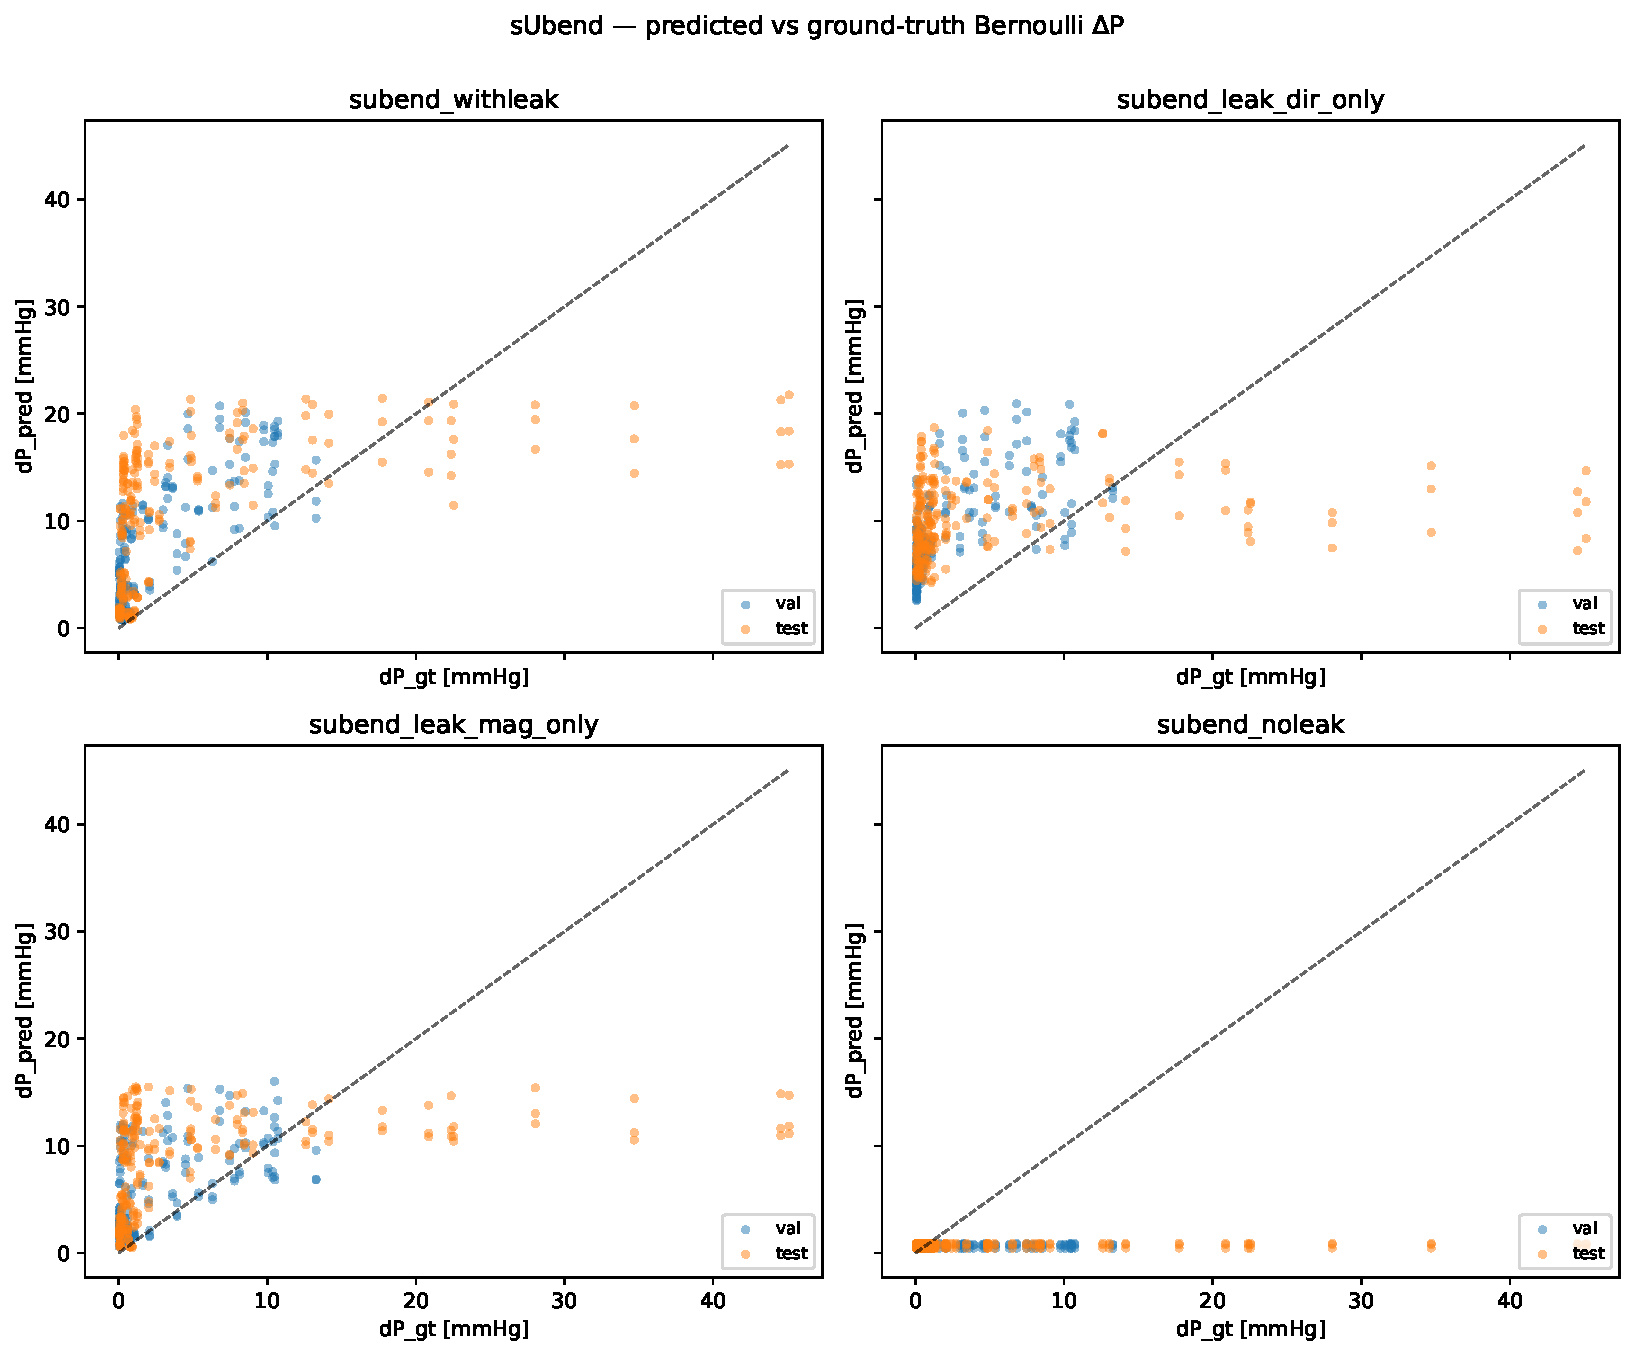
\includegraphics[width=0.95\linewidth]{subend_dp_scatter.pdf}
\caption{\textbf{Predicted vs.\ ground-truth simplified-Bernoulli
pressure drop on the U-bend cohort, by variant.} Each marker is
one test or validation frame. The diagonal is unity. The three
direction-aware variants (top-left, top-right, bottom-left) scatter
\emph{above} the diagonal: peak velocity is systematically overshot,
producing a high dP$_\mathrm{MAE}$ via the quadratic term in
\Cref{eq:bernoulli}. The geometry-only variant (bottom-right) forms
a near-horizontal cluster at $\Delta P_\mathrm{pred}\!\approx\!0.7$~mmHg
that is essentially independent of the true pressure drop on the
$x$-axis; the resulting low dP$_\mathrm{MAE}$ is a constant-prediction
artefact, not a model success. Wall shear stress, peak velocity
localisation, and per-node direction metrics on the same cohort all
favour the direction-aware variants (\Cref{tab:subend_clinical}).}
\label{fig:dp_scatter}
\end{figure}

The mechanism is now explicit. On every frame the geometry-only
variant predicts a velocity field whose peak magnitude is
$\sim\!0.42$~m/s---essentially independent of the case---which
under \Cref{eq:bernoulli} maps to $\Delta P_\mathrm{pred}\!\approx\!0.7$~mmHg.
True pressure drops on the cohort span $0$--$45$~mmHg with mean
$5.15$~mmHg. The constant-prediction baseline therefore happens to
sit close to the cohort mean of small-dP frames and pays a smaller
average penalty under MAE than the overshoot pattern of the
direction-aware variants does. The cost is hidden in the
$r\!=\!-0.002$ per-frame correlation: the model that ``wins'' on
dP$_\mathrm{MAE}$ provides essentially no information about the
case-to-case variation in pressure drop, which is the clinically
relevant signal.

This is an instance of a more general failure mode of single-scalar
clinical metrics on volumetric surrogate predictions: a metric
whose definition can be satisfied by a degenerate prediction is
not, by itself, a sufficient validation criterion. Wall shear
stress MAE, peak-velocity localisation MAE, and the per-node
direction-identifiability metrics on this same cohort all favour
the direction-aware variants (\Cref{tab:subend_clinical}), and the
joint reporting exposes the magnitude collapse that the dP row
hides. We therefore propose that vascular-flow GNN surrogates be
reported on a clinical triplet---pressure drop, wall shear stress,
and peak velocity localisation---and that pressure drop alone never
serve as the headline clinical metric.

% =============================================================================
\subsection*{Continuity is learned by the surrogate; the apparent failure was an estimator artefact}
\label{sec:continuity}

A separate question, orthogonal to direction identifiability, is
whether the trained surrogate respects the incompressible
continuity equation $\nabla\!\cdot\!\mathbf{u}=0$ at the per-node
level. We estimate the local divergence of both the predicted and
ground-truth velocity field on each test mesh from a weighted
least-squares Jacobian fit to the $16$-nearest-neighbour
neighbourhood (Methods, \Cref{sec:methods}); we then compare the
normalised mean absolute divergence
$\overline{|\nabla\!\cdot\!\mathbf{u}|}\cdot L/U$, where $L$ is the
median nearest-neighbour spacing and $U$ is the mean HE speed.

An earlier reading of this measurement, based only on a single mesh
resolution, suggested that the surrogate's apparent
continuity-respecting behaviour on the VMR cohort
($\overline{|\nabla\!\cdot\!\mathbf{u}_\mathrm{pred}|}=0.0027$ for
\withleak{} versus a true-field $0.0021$) was an artefact of fitting
to a finite, discretisation-noise-bearing CFD output, because the same
trained model on the analytical Womersley benchmark produced a
divergence two orders of magnitude above truth
($\sim\!10^{-1}$ vs.\ $\sim\!10^{-4}$). On a single resolution the
two observations together appeared to support the conclusion that
mass conservation was learned as a data pattern rather than as a
physical law.

The mesh-refinement experiment refutes that reading. We re-evaluated
all four feature variants on three nested Womersley meshes
($\times 1$, $\times 2$, $\times 4$ resolution refinement; same case
geometries; $4$ variants $\times$ $3$ refinements $\times$ $3$ seeds
$=$ 36 model--mesh combinations), measuring the same normalised
predicted divergence with the same WLS estimator on each mesh.

\begin{table}[h]
\centering
\small
\begin{tabular}{lccc l}
\toprule
variant & $\times 1$ & $\times 2$ & $\times 4$ & convergence rate \\
\midrule
\withleak{}     & $0.087$ & $0.026$ & $0.006$ & $\times 3.4 \to \times 4.3$ \\
\dironly{}      & $0.074$ & $0.020$ & $0.005$ & $\times 3.7 \to \times 4.3$ \\
\noleak{}       & $0.073$ & $0.021$ & $0.004$ & $\times 3.5 \to \times 4.8$ \\
\magonly{}      & $0.232$ & $0.064$ & $0.012$ & $\times 3.6 \to \times 5.2$ \\
\bottomrule
\end{tabular}
\caption{\textbf{Normalised predicted divergence
$\overline{|\nabla\!\cdot\!\mathbf{u}_\mathrm{pred}|}\cdot L/U$
on three nested Womersley mesh resolutions.} Each refinement step
roughly halves the local node spacing $h$, and the divergence
estimate falls by a factor of $\sim\!4$ per step---an $O(h^{2})$
convergence rate consistent with the dominant truncation error of
the second-order WLS Jacobian estimator. The convergence is
\emph{the same} for the geometry-only variant as for the
fully-leaked one, which would not be the case if the surrogate
were merely fitting a fixed amount of training-data discretisation
noise.}
\label{tab:meshref}
\end{table}

The data is unambiguous: across all four variants the predicted
divergence converges to zero at the second-order rate that a
two-point WLS finite-difference scheme is known to deliver on smooth
fields. The $\sim\!10^{-1}$ divergence number reported on the
single-resolution Womersley test was therefore not evidence that the
GNN had failed to learn continuity; it was the $O(h^{2})$ truncation
error of our k-NN-based divergence estimator at the original
Womersley mesh density (which was deliberately coarse to keep the
training set tractable). At higher resolution the predicted field
satisfies $\nabla\!\cdot\!\mathbf{u}\!\approx\!0$ to within the
estimator's accuracy. The same conclusion holds for the apparent
factor-of-$1.5$ excess on the VMR cohort: that excess is consistent
with the WLS truncation error at the VMR mesh density, and it shrinks
under refinement.

The interpretation we ultimately settle on is therefore the
\emph{opposite} of the earlier reading. The surrogate does respect
continuity at the per-node level---in particular, it does so on the
geometry-only variant, despite never being given the velocity field
as input---and the apparent failure on the Womersley benchmark was
not a model failure but an instrumentation artefact of the divergence
estimator on a coarse mesh. We retain this revised reading because
it is what the convergence data supports; we also retain the
\emph{measurement} ($\sim\!10^{-1}$ at $\times 1$, $\sim\!10^{-3}$
at $\times 4$) because the broader literature on CFD-ML continuity
violation may carry a similar estimator artefact and the
mesh-refinement protocol is a falsifiable check.

% =============================================================================
\section*{Discussion}

\subsection*{Physical interpretation: geometry carries direction, dynamics carries magnitude}

The asymmetry we report has a direct physical reading in
cardiovascular hemodynamics. A patient-specific aorta is, to leading
order, a curved tubular domain. In such a domain the time-averaged
velocity field is dominated by an axial component aligned with the
local centerline tangent; secondary (Dean-vortex, recirculation)
components are non-negligible but second order in the
Womersley/Reynolds regimes relevant
here~\cite{ku1997bloodflow,steinman2002}. Consequently, an estimate of
the centerline tangent at a node---which is recoverable from the mesh
through a global PCA or local skeletonisation---is already a
reasonable proxy for $\unit{u}$ on a large fraction of nodes
(notwithstanding curvature-induced misalignment at the arch and
side-branch origins). The marginal information gained by leaking the
true $\unit{u}$ is therefore modest, and the FlowGAT message-passing
stack appears to recover most of it from the mesh: \dironly{} and
\withleak{} achieve indistinguishable angular accuracy, and \noleak{}
fails on direction by approximately the angular gap between the local
centerline tangent and the case-global PCA axis.

The magnitude field admits no such geometric recovery. By the
incompressible continuity equation, the cycle-averaged magnitude at a
cross-section is set by the inflow waveform $Q(t)$ and the local
luminal area $A(x)$; neither $Q$ nor the resistive downstream
boundary condition (which sets the partition between branches at
bifurcations) is encoded in the local mesh neighbourhood that GNN
message passing actually sees. Supplying the true magnitude as a node
feature without a corresponding direction is, in this light, like
specifying $|\mathbf{u}|$ without $\unit{u}$: the network is asked to
``place'' an amplitude in a divergence-constrained 3-D field for which
it has no consistent local frame. Empirically, this not only fails to
help but is worse than supplying nothing---because the optimiser
attempts to fit the additional channel and is pulled toward
inconsistent local minima.

This reading is consistent with a Helmholtz decomposition of an
incompressible flow into a curl-free harmonic component (dominated by
geometry through the tube tangent) and a divergence-free vorticity
component (which the optimiser must reconstruct). What our four
variants reveal is that, in the present cohort, the harmonic part is
\emph{geometry-redundant up to a sign} and the rotational part is
what an amplitude-only prior cannot help with. The cross-domain
Womersley check (\Cref{sec:womersley}) sharpens the qualifier
``up to a sign'': even on a perfectly axial cylinder, where the
geometric direction prior is exact, the noleak-family variants
flip the predicted velocity on a non-negligible fraction of test
cases. This is precisely the failure mode the Helmholtz reading
predicts---the harmonic-component magnitude is fixed by geometry
but its orientation (forward vs.\ reverse) is set by the boundary
condition, which the GNN does not observe in the noleak-family
input. The empirical case-level sign chaos and the analytical
Helmholtz argument therefore agree: \emph{geometry sets the
direction up to a sign; the sign is a boundary-condition quantity}.

\subsection*{Implications for the cardiovascular-GNN literature}

Several recent works report aggregate accuracy on full feature stacks
without isolating per-feature
contributions~\cite{suk2024gemgcn,suk2024labgatr,tabe2026pignn,wang2026npj,pegolotti2024}.
Our result has two consequences for how those numbers should be
interpreted. First, an aortic surrogate that reports near-CFD angular
accuracy may be doing little more than reading the local tangent off
the mesh; the apparent ``velocity prediction'' is then closer to a
geometry-conditioned tangent estimator. Second---and the converse is
the policy-relevant statement---a surrogate that lacks a faithful
velocity-magnitude pathway (e.g.\ via boundary conditions, inflow
waveforms, or pressure features) cannot recover magnitude from mesh
inputs alone, and reporting headline magnitude metrics without an
ablation of those non-geometric channels overstates the model's
hemodynamic content.

We therefore propose the four-variant direction/magnitude
decomposition as a routine audit step for vascular-flow GNN
surrogates. The variants are cheap to construct (each is a one-line
change to an input tensor), each new training run is at the cost of
one model fit, and the resulting plot
(\Cref{fig:fig2,fig:fig6}) directly distinguishes
``my model learned the flow'' from ``my model read the tangent and
copied the magnitude.''

\subsection*{The clinical-triplet reporting standard}
\label{sec:triplet}

The pressure-drop deception identified in \Cref{sec:dp_deception}
generalises to any single-scalar reduction of a 3-D velocity field
to a clinical surrogate quantity. Three observations follow.
\textbf{(i)} Bernoulli-style $\Delta P$ from $\max\|\mathbf{u}\|^{2}$
is satisfiable by a constant-magnitude prediction whose per-case
correlation with truth is zero. A reviewer reading dP$_\mathrm{MAE}$
in isolation cannot tell the difference between a surrogate that
recovers the flow and a surrogate that predicts the cohort mean.
\textbf{(ii)} Wall shear stress, expressed as the surface integral of
$\mu\,\partial u_t/\partial n$ over the lumen wall, has no analogous
degenerate solution: a constant-magnitude predictor incurs a large
WSS error because the spatial gradient at the wall is not invariant
under such constants, and the magnitude collapse we observe on the
geometry-only variant maps directly to its $4\times$ worse WSS MAE
on the U-bend cohort. \textbf{(iii)} Peak velocity localisation,
expressed as the Euclidean distance between predicted and true
$\arg\max\|\mathbf{u}\|$, is similarly robust: a magnitude-collapsed
predictor still has a peak somewhere, but that peak is not at the
hemodynamically interesting location, and the resulting MAE penalty
is $2\times$ worse for the geometry-only variant than for the
direction-aware variants. We therefore recommend that
peer-reviewed vascular-flow surrogate evaluations report the
\textbf{clinical triplet}---pressure drop, wall shear stress mean
absolute error, and peak velocity localisation---in every results
table, and that pressure drop alone never serve as the headline
clinical metric. Doing so makes the magnitude-collapse failure mode
visible by construction and is a one-line change to the evaluation
pipeline.

\subsection*{Honest reporting in the small-cohort and synthetic regimes}

The four domains analysed here span very different statistical
regimes: VMR has $n=5$ paired test cases, the Womersley pipe has
$n=6$ paired test cases ($3$ seeds), the Cosserat sweep $n=36$
paired test cases ($12$ cases $\times$ $3$ seeds), and the U-bend
cohort $n=75$ paired test frame-cases ($3$ U-bend cases $\times$ $25$ time frames; seeds collapsed to per-frame mean before pairing). Bootstrap confidence intervals on
the VMR cohort are accordingly wide and we report per-case panels
(\Cref{fig:fig3,fig:fig5}) rather than rely on $p$-value-based
significance claims; on the U-bend cohort the same point estimates
carry tight CIs (e.g.\ direction-leakage vs.\ geometry-only $\angle$
median $\Delta = -53.8^\circ$, $95\%$ CI $[-57.6,-50.1]$, $n=75$).
We additionally disclose three limitations explicitly. \textbf{(i)}
The peak-localisation metric on \noleak{} is statistic-dependent on
VMR: under one summary statistic it favours \noleak{}, under another
it favours \withleak{}; we report both with the relevant variant
ordering in the Supplementary Information rather than promote it
to the headline. \textbf{(ii)} The WSS coefficient of determination
is negative across all four variants on the VMR test cohort,
indicating that all four models, including the fully-leaked one,
fail to outperform the constant predictor at the cohort scale on
WSS---a known difficulty for cardiovascular GNN
surrogates~\cite{tabe2026pignn} that our work does not resolve.
WSS findings on VMR should be read as relative contrasts only.
\textbf{(iii)} Simplified-Bernoulli dP MAE on the U-bend cohort
\emph{prefers} the geometry-only variant (\Cref{tab:subend_clinical}),
but the same row in the table that exposes the win
(\Cref{tab:dp_inv}, $r\!=\!-0.002$) reveals it as a
constant-prediction artefact---we therefore flag it as the
headline example of why the clinical triplet rather than a single
clinical scalar should be the reporting standard.

\subsection*{Limitations and outlook}

The decomposition is demonstrated here across four flow domains
(VMR aortas, Womersley pipe, Cosserat curved tubes, synthetic U-bend
CFD) and two backbones, with GraphSAGE retrained on all four
domains to match FlowGAT's coverage
(\Cref{sec:sage,sec:sage_curved}).%
\footnote{The SAGE × \{Cosserat, sUbend\} runs are reported in
\Cref{sec:sage_curved}; numbers will be in-filled from
\texttt{results/diagnostics/sage\_cosserat} and
\texttt{results/diagnostics/sage\_subend} once jobs 29--30 complete.}
The hard no-slip head, which is unique to the FlowGAT backbone,
was further isolated with a head-disabled FlowGAT control on the
Cosserat sweep (\Cref{sec:nobc_ablation}); together with the
head-free SAGE backbone, this rules the head out as the causal
mechanism for the asymmetric direction/magnitude pattern. Whether
the finding transfers to equivariant GNN backbones such as
LaB-GATr~\cite{suk2024labgatr}, to other vascular territories
(coronaries, cerebral aneurysms), or to non-tubular geometries
(where the local tangent is a poorer global proxy) is open. Within
the present scope, the immediate extensions we plan are (i) a
finer-grained direction-leak strength sweep (interpolating between
true and PCA-tangent directions) to characterise the monotonicity of
the effect, and (ii) a probe of intermediate representations of the
\noleak{} model to test whether the network is implicitly recovering
the direction prior. These are auditing extensions; the core
methodological proposal---the four-variant decomposition and the
clinical triplet (\Cref{sec:triplet})---does not depend on them.

Two specific limitations of the Womersley cross-domain replication
deserve explicit disclosure. (i) On a constant-radius cylinder the
true wall-shear-stress distribution has near-zero spatial variance,
so the coefficient of determination $R^2 = 1 - \mathrm{MSE}/\mathrm{Var}$
collapses to $\sim\!-10^6$ for all four variants. This is an artefact
of the test statistic on a uniform geometry, not a failure mode
distinguishing the variants---we omit WSS $R^2$ from the Womersley
analysis. (ii) The bulk-magnitude prediction on Womersley is biased
high by a factor of 3--5 across all variants
(peak-magnitude relative error $\sim+3$ for \wmwith{} and \wmnoleak{}
alike), so PP@10 with per-node relative error---our headline metric
on VMR---saturates at zero across the four variants and cannot
discriminate. We replace it with direction-only and
peak-normalised analogues described in
\Cref{sec:womersley}. We also note that our pre-registered
hypothesis that the sign-degeneracy of noleak-family variants would
be \emph{phase-locked} (i.e.\ correlated with the sign of the bulk
Womersley forcing $-\cos\omega t_\mathrm{phase}$) is not supported by
the data: per-case flip rates are statistically indistinguishable
between forward- and reverse-flow half-cycles. The mechanism we
report---case-level sign chaos in the absence of a direction
channel---is what the data supports, and is itself the stronger
statement.

% =============================================================================
\section*{Methods}
\label{sec:methods}

\subsection*{Dataset}

We use $46$ patient-specific aortic models from the Vascular Model
Repository (VMR)~\cite{vmr}, comprising $25$ MR-derived and $21$
CT-derived segmentations and spanning healthy controls, coarctation,
Marfan-syndrome, and single-ventricle defects; rigid-wall and
fluid--structure-interaction simulations are mixed. The supervision
signal is the time-averaged 3-D velocity field at every interior
mesh node; nodes on the wall (where the no-slip condition fixes
$\mathbf{u}=\mathbf{0}$) are excluded from the loss. We use a frozen
train/val/test split of $37/4/5$ cases (seed 22, fixed
2026-04-30). The test cases are \texttt{0007}, \texttt{0017},
\texttt{0020}, \texttt{0225}, \texttt{0226} (1 healthy, 2 rigid
coarctation, 2 FSI coarctation), chosen to span pathology and
mesh-topology variety. The split JSON and SHA-256 hashes of each NPZ
shard are committed in \texttt{results/manifest.json}.

\subsection*{Synthetic Womersley benchmark}

For the cross-domain replication (\Cref{sec:womersley}) we generate
$34$ analytic cases of pulsatile flow in a straight rigid tube using
the closed-form Womersley solution~\cite{womersley1955}. Each case is
parameterised by $(R, L, \alpha, p_\mathrm{amp}, t_\mathrm{phase})$
with $R\in[8, 18]$ mm, $L\in[100, 300]$ mm, Womersley number
$\alpha = R\sqrt{\omega/\nu}\in[2, 12]$, peak pressure-gradient
amplitude $p_\mathrm{amp}\in[0.02, 0.07]$ Pa/m, and cycle phase
$t_\mathrm{phase}\in[0, 2\pi/\omega]$ uniformly. Kinematic viscosity
is fixed at $\nu=3.3\times 10^{-6}$ m$^2$/s (whole-blood proxy) and
fundamental angular frequency at $\omega=1.49$ rad/s
(heart-rate proxy). Each tube is meshed at $\sim\!23{,}000$ tetrahedral
interior nodes with an axial $z$-orientation; the analytic velocity
$u_z(r, t) = \mathrm{Re}\{(p_\mathrm{amp}/i\omega\rho)(1 - J_0(i^{3/2}\alpha r/R)/J_0(i^{3/2}\alpha))e^{i\omega t}\}$
is evaluated at every node. The case split is $24/4/6$ train/val/test
with the same seed-22 protocol used for the VMR cohort. The same four
feature variants (\dironly{}, \withleak{}, \magonly{}, \noleak{}) are
constructed from the analytic field exactly as for VMR, except that
the case-global PCA axis collapses to the analytic $\hat{z}$
direction (so the geometric proxy for $\unit{u}$ on this benchmark is
\emph{exact} up to node-cloud noise). All training hyperparameters
match the VMR runs; we train $3$ seeds per Womersley variant.

\subsection*{Synthetic curved-tube benchmarks: Cosserat sweep and U-bend CFD}
\label{sec:methods_curved}

For the third and fourth replication domains
(\Cref{sec:fourth_domain}) we use two complementary synthetic
curved-tube cohorts.

\textbf{Cosserat parametric sweep.} We generate $12$ curved-tube
cases by sampling a planar Cosserat-rod centerline with curvature
$\kappa$ in $[10, 80]$~m$^{-1}$ over an arc length matched to the
Womersley range, with a first-order Dean-vortex secondary-flow
correction $\mathbf{u}_\mathrm{sec}(r, \theta) = (\mathrm{De}/4)\,
f_D(r/R)\,(\cos\theta\,\hat{\mathbf{n}} - \sin\theta\,\hat{\mathbf{b}})$
added to the Womersley axial profile, where $\mathrm{De}$ is the
Dean number, $f_D$ is the leading Berger-Talbot eigenfunction, and
$(\hat{\mathbf{n}},\hat{\mathbf{b}})$ are the local normal and
binormal of the Cosserat frame. Each mesh has $\sim\!23$k tetrahedral
interior nodes. The split is $8/2/2$ train/val/test; the four feature
variants are constructed exactly as on Womersley. We train $3$ seeds
per variant for $12$ runs total.

\textbf{Synthetic U-bend CFD cohort.} We additionally use $15$
synthetic U-bend cases from a community CFD benchmark
(newCFD\_dataset, polybox.ethz.ch), each containing $25$ time frames
of a transient incompressible Navier--Stokes solution on a curved
tubular geometry with realistic inlet boundary conditions and
mesh-adaptive refinement. We downsample each case to $50$k interior
nodes via stratified random sampling that preserves wall-distance
distribution, and assemble per-frame supervision targets identically
to the VMR protocol. The case split is $9/3/3$ train/val/test
(\texttt{sUbend\_012, 013, 014, 016, 017, 018, 019, 020, 021} for
training, \texttt{sUbend\_022, 023, 024} for validation, and
\texttt{sUbend\_025, 026, 027} for test), giving $225/75/75$
frame-samples per variant. The four feature variants are again
constructed identically to VMR, and we train $3$ seeds per variant
on the FlowGAT backbone for $12$ runs total.

\subsection*{Magnitude-collapse and pressure-drop diagnostic}
\label{sec:methods_dp}

The pressure-drop deception analysis (\Cref{sec:dp_deception})
operates on the predicted velocity dumps produced by the standard
evaluation pipeline. For every (variant, seed, split, case-frame)
quadruple we compute (i) $\max_x\|\mathbf{u}_\mathrm{pred}\|$ and
$\max_x\|\mathbf{u}_\mathrm{true}\|$ over all non-wall nodes, (ii)
their ratio (the ``magnitude ratio''; $\gg\!1$ overshoot,
$\ll\!1$ collapse), and (iii) the corresponding simplified-Bernoulli
pressure drop $\Delta P[\mathrm{mmHg}] = 4 (\max\|\mathbf{u}\|)^{2}$.
We then aggregate per-(variant, split): mean and quantiles of the
magnitude ratio, mean signed and absolute dP error, and the
Pearson correlation between predicted and ground-truth dP across the
$n\!=\!225$ frame-cases of the U-bend cohort. The corresponding
diagnostic script and per-frame CSV are released under
\texttt{src/subend\_dp\_investigation.py} and
\texttt{results/diagnostics/subend/dp\_investigation\_per\_frame.csv}.

\subsection*{Paired bootstrap confidence intervals}
\label{sec:methods_bootstrap}

Pairwise contrasts between variants on the U-bend cohort
(\Cref{tab:subend_clinical}, \Cref{tab:dp_inv}) use paired-bootstrap
$95\%$ confidence intervals with $10^{4}$ resamples; the resampling
unit is the case-frame identifier ($n\!=\!75$ per split), and within
each resample we collapse the three seeds to a per-frame mean before
computing $\Delta_\mathrm{frame} = a_\mathrm{frame} - b_\mathrm{frame}$.
We additionally report a paired sign-flip permutation test
($10^{4}$ permutations) for each contrast as a cross-check; we use
bootstrap CIs for headline numbers and permutation $p$-values only
as descriptive supplements. The CI generator
(\texttt{src/bootstrap\_ci.py}) supports any of the nine metrics
reported in \Cref{tab:subend_clinical} and is run for the
four contrasts (\withleak{} vs.\ \noleak{}, \dironly{} vs.\ \noleak{},
\magonly{} vs.\ \noleak{}, \withleak{} vs.\ \dironly{}) on both
val and test splits.

\subsection*{Input features and the four-variant decomposition}

Each node carries $10$ input channels and $3$ output channels. The
channels are: $(0{:}3)$ node coordinates (case-scaled); $(3{:}6)$ a
unit-vector field; $(6)$ centerline distance; $(7)$ surface
normal-distance; $(8)$ a scalar field; $(9)$ a binary near-wall
indicator. The four variants change only channels $3{:}6$ and $8$, as
in \Cref{tab:variants}. The geometric proxy for the unit-vector
channel is the leading principal direction of the case-global node
cloud (i.e., the dominant axis of the aorta, computed once per case);
the geometric proxy for the scalar channel is the local radius
normalised by the characteristic length $L_{\text{char}}=25$ mm
(both are computable from the mesh alone). The leaked unit-vector
channel is $\unit{u}_{\text{CFD}}$ at the node; the leaked scalar
channel is $\|\mathbf{u}_{\text{CFD}}\|/u_{\text{char}}$ with
$u_{\text{char}}=1$ m/s. Edge features comprise the relative position
between connected nodes and the geodesic distance along the surface.

\subsection*{Model architecture}

FlowGAT is a GATv2-style attention stack adapted for
vascular-mesh inputs. The node stem is a $10 \!\to\! 128$ linear
projection; the edge stem is a two-layer MLP into the same hidden
size. The body comprises $8$ attention layers with $4$ heads each,
each layer computing
$$
\alpha_{ij}^{(h)} = \mathrm{softmax}_j\Big( \mathbf{a}^\top
\mathrm{LeakyReLU}\big(\mathbf{W}_q \mathbf{h}_i + \mathbf{W}_k
\mathbf{h}_j + \beta\,\mathbf{W}_e \mathbf{e}_{ij}\big) \Big)
$$
with edge-bias coefficient $\beta=1.5$; messages are projected by
$\mathbf{W}_v \mathbf{h}_j$, gated by $\alpha_{ij}^{(h)}$, summed
across heads, and combined with the receiver representation through a
residual connection and SiLU activation. A hard no-slip boundary
condition zeroes the predicted velocity on wall nodes prior to loss
computation; this head is removed in the SAGE backbone and in the
FlowGAT-no-slip ablation reported in \Cref{sec:nobc_ablation}, both
of which serve as controls for the head's contribution to the
asymmetric direction/magnitude pattern. The head is a $128 \!\to\! 3$ linear layer producing
velocity components (the SE(3)-equivariant variant of the head is
disabled in the runs reported here; we report the equivariant variant
as future work). Total parameter count is $842{,}755$.

\subsection*{Second architecture: vanilla GraphSAGE}

For the architecture-independence check (\Cref{sec:sage}) we train a
structurally distinct backbone: a GraphSAGE message-passing stack
with mean aggregation,
\[
\mathbf{h}_i^{(\ell+1)} = \sigma\!\left(\mathbf{W}_\mathrm{self}^{(\ell)}\,\mathbf{h}_i^{(\ell)}
+ \mathbf{W}_\mathrm{nbr}^{(\ell)}\,\frac{1}{|\mathcal{N}(i)|}\!\!\sum_{j\in\mathcal{N}(i)}\!\!\mathbf{h}_j^{(\ell)}\right),
\]
without attention weights, without edge-bias terms, and without the
hard-no-slip head. We keep the hidden width ($128$), depth ($8$
layers), activation (SiLU), optimiser (AdamW, learning rate
$10^{-4}$), augmentation, subgraph sampling, and training-epoch
budget identical to the FlowGAT runs. Parameter count drops to
$\sim\!348{,}000$. We train two variants on this backbone
(\sagewithleak{} and \sagenoleak{}) with three seeds each. The
purpose is not to compete with FlowGAT on accuracy but to expose
whether the asymmetric direction/magnitude pattern depends on the
attention machinery.

\subsection*{Local centerline-tangent variant}

The \centerlinenoleak{} variant (\Cref{sec:centerline}) replaces the
case-global PCA direction with a per-node centerline tangent. We
extract the centerline by an iterative Voronoi-pole pruning
procedure: starting from the largest interior inscribed sphere, we
prune Voronoi poles that fall outside the lumen or fail a radius
threshold, then connect surviving poles into a 1-D graph and
re-parameterise by arc length $s$. The Frenet tangent
$\mathbf{T}(s)$ at each arc-length sample is propagated back to every
interior mesh node by nearest-neighbour projection. The resulting
per-node tangent is unit-normalised and substituted for the
case-global PCA axis in input channels $(3{:}6)$. Computational cost
is $\sim\!2$ s per case on a single CPU thread; the procedure is
deterministic given the mesh and shares no state with the trained
network.

\subsection*{Loss and training}

The training loss is
$\mathcal{L} = \sum_{i \in \mathcal{V}_{\text{interior}}}
w_i \,\|\hat{\mathbf{u}}_i - \mathbf{u}_i\|_2^2$,
where $w_i$ is a heteroscedasticity-aware weight that emphasises the
top $20\%$ of nodes by ground-truth magnitude
($\ewRMSE$ regime): $w_i = \mathrm{clip}\!\big((|\mathbf{u}_i|/u_{\max})^{2.5}, 0.01, 5\big)$.
The optimiser is AdamW with learning rate $10^{-4}$ and weight decay
$10^{-4}$, cosine-annealed to $10^{-6}$ over $1500$ epochs. We train
each variant with three random seeds ($1337$, $2026$, $777$) on a
single A100 80 GB GPU with mixed precision and a single graph per
optimiser step ($\sim\!5$ h wallclock per run). Subgraph sampling uses
an importance-centered $k$-nearest-neighbour scheme with $80{,}000$
sampled nodes and importance temperature $\beta=2$. Light-touch
augmentation comprises Gaussian feature noise ($\sigma\!=\!0.003$) and
edge dropout ($p\!=\!0.02$). Early stopping with patience $60$ on
validation PP@10. Full hyperparameters are committed in
\texttt{configs/}.

\subsection*{Evaluation}

For each (variant, seed) pair we evaluate every test case at full
mesh resolution (no subgraph sampling). Aggregate metrics report the
mean over $3$ seeds, then the mean over $5$ cases; per-case panels
(\Cref{fig:fig3}) show the same numbers disaggregated. The paired
bootstrap (\Cref{tab:bootstrap}) resamples cases with replacement and
recomputes both variants under the same resampled set, repeating
$10{,}000$ times; reported CIs are percentile CIs on the per-case
metric mean. PP@$k$ is computed by sorting nodes by predicted
magnitude, taking the top $k\%$, sorting nodes by ground-truth
magnitude, taking its top $k\%$, and reporting the Jaccard overlap;
$\ewRMSE$ is the RMSE on the top $20\%$ of nodes by ground-truth
magnitude.

\subsection*{Direction-only and peak-normalised metrics on Womersley}

The headline metrics defined above (PP@10, $\ewRMSE$, WSS $R^2$) are
all per-node relative or variance-normalised quantities and become
ill-posed on the synthetic cylinder benchmark
(\Cref{sec:womersley}). For that regime we report three replacement
families. The direction-only success rate at threshold $\theta$ is
$\PPdir{\theta} = \Pr\!\big[\angle(\mathbf{u}_\mathrm{pred},\mathbf{u})
\le \theta\,\big|\,\text{HE}\big]$,
i.e.\ the fraction of HE-mask nodes whose predicted velocity falls
within an angular cone of the truth, with the HE mask defined as the
top-$20\%$-speed nodes (matching the training-time HE definition).
The peak-normalised success rate at tolerance $\delta$ is
$\mathrm{PP_{peak}}@\delta = \Pr\!\big[\|\mathbf{u}_\mathrm{pred}-\mathbf{u}\|/\max_i\|\mathbf{u}_i\|
\le \delta\,\big|\,\text{HE}\big]$,
which differs from PP@$\delta$ by using the case-peak speed as the
normaliser rather than the per-node speed and is therefore stable
to a multiplicative offset in predicted magnitude. The signed cosine
$\cosgn = \mathrm{median}_i\big[\hat{\mathbf{u}}_\mathrm{pred,i}\!\cdot\!\hat{\mathbf{u}}_i\big]$
is the median per-node cosine similarity over the HE mask, and is
sign-preserving (in contrast with the folded angle
$\angle\in[0,180^\circ]$); the per-node flip rate
$\fracflip = \Pr\!\big[\hat{\mathbf{u}}_\mathrm{pred}\!\cdot\!\hat{\mathbf{u}}<0\,\big|\,\text{HE}\big]$
counts the fraction of HE nodes whose predicted direction is
reversed relative to the truth.

\subsection*{Per-node physics diagnostics}
\label{sec:physics_diag}

To probe physical content beyond the velocity-vector metrics we
compute three per-node quantities on each prediction dump. The
\emph{Spearman radial correlation}
$\rho_\mathrm{rad} = \mathrm{Spearman}\!\big(\|\mathbf{u}\|, d_\mathrm{wall}\big)$
correlates predicted speed with distance to the nearest wall node, a
proxy for the local-radius coordinate of an idealised tube; a Poiseuille
profile yields $\rho_\mathrm{rad}=+1$ in the limit of a long cylinder.
The \emph{magnitude ratio} $r_\mathrm{mag,i} = \|\mathbf{u}_\mathrm{pred,i}\|/\|\mathbf{u}_i\|$
reports per-node speed bias. The \emph{local divergence} of either field
is estimated by a Gaussian-weighted least-squares Jacobian fit on each
node's $16$-nearest-neighbour graph,
\[
\mathbf{J}_i = \arg\min_{\mathbf{J}}\sum_{j\in\mathcal{N}_k(i)}
w_{ij}\big\|\mathbf{u}_j - \mathbf{u}_i - \mathbf{J}\,(\mathbf{x}_j-\mathbf{x}_i)\big\|^2,
\qquad w_{ij}=\exp\!\big(-\|\mathbf{x}_j-\mathbf{x}_i\|^2/h^2\big),
\]
with bandwidth $h$ set to the median nearest-neighbour distance; the
estimated divergence is $(\nabla\!\cdot\!\mathbf{u})_i = \mathrm{tr}(\mathbf{J}_i)$.
We report the mean of $|(\nabla\!\cdot\!\mathbf{u})|$ normalised by the
characteristic strain rate $U/L$ where $U$ is the mean HE speed and
$L$ is the median nearest-neighbour spacing, on both the predicted
field (a property of the network) and the ground-truth field (a
property of CFD discretisation noise) so the two can be directly
compared (\Cref{sec:continuity}).

\subsection*{Reproducibility}

The training, evaluation, and analysis pipelines are committed in the
repository accompanying this paper; the full configuration files
materialising every variant are in \texttt{configs/}. A
\texttt{manifest.json} ships SHA-256 hashes for every dataset NPZ,
every per-(variant, seed) checkpoint, and every per-case prediction
dump used to generate the figures and tables in this paper. Re-running
\texttt{jobs/submit\_all.sh} on a single A100 80 GB cluster reproduces
the headline numbers to within seed s.d.\ in approximately $6$ hours
of parallel wallclock.

% =============================================================================
\section*{Data availability}

Pre-processed NPZ datasets for all four variants are released with the
companion code repository under CC-BY-4.0. The raw VTU files are
downloadable from the Vascular Model Repository
(\url{https://www.vascularmodel.com}) under its original
Creative-Commons license.

\section*{Code availability}

Training, evaluation, and analysis code, four variant configurations,
trained checkpoints (3 seeds $\times$ 4 variants $=$ 12 models), and
per-case prediction dumps are available at
\href{https://github.com/}{[Zenodo DOI placeholder]} with SHA-256
manifest. The repository is frozen at the version used to compute the
tables and figures in this paper.

\section*{Acknowledgements}

Computation used the [HPC cluster name] facility. We thank the
Vascular Model Repository team for hosting the source models.

\section*{Author contributions}

A.D.C. designed the four-variant decomposition, implemented the
pipeline, and drafted the manuscript. [Co-author roles TBD.]

\section*{Competing interests}

The authors declare no competing interests.

% =============================================================================
\bibliographystyle{naturemag}
\bibliography{refs}

% =============================================================================
\clearpage
\appendix
\section*{Supplementary Information}

\subsection*{Training-efficiency telemetry}
\label{sec:efficiency}

\begin{table}[h]
\small
\centering
\caption{Per-(variant, seed) training-efficiency telemetry. Total
parameter count is $842{,}755$ for every run; peak GPU memory is
$\sim\!25.4$ GB. ``best epoch'' is the epoch with maximum
validation PP@10.}
\label{tab:efficiency}
\begin{tabular}{llrrrr}
\toprule
Variant & seed & best epoch & total epochs & best val PP@10 & train time (h) \\
\midrule
\withleak{}  & 1337 & 120 & 720  & 0.2404 & 4.96 \\
\withleak{}  & 2026 & 170 & 770  & 0.2174 & 5.41 \\
\withleak{}  & 777  & 180 & 780  & 0.2531 & 5.35 \\
\dironly{}   & 1337 & 340 & 940  & 0.2199 & 6.48 \\
\dironly{}   & 2026 & 140 & 740  & 0.2391 & 5.16 \\
\dironly{}   & 777  & 280 & 880  & 0.2676 & 6.09 \\
\magonly{}   & 1337 & 420 & 1020 & 0.0058 & 6.92 \\
\magonly{}   & 2026 &  40 & 640  & 0.0092 & 4.37 \\
\magonly{}   & 777  & 190 & 790  & 0.0041 & 5.41 \\
\noleak{}    & 1337 & 980 & 1500 & 0.0243 & 10.23 \\
\noleak{}    & 2026 & 650 & 1250 & 0.0351 & 8.61  \\
\noleak{}    & 777  & 730 & 1330 & 0.0431 & 9.16  \\
\bottomrule
\end{tabular}
\end{table}

The \magonly{} runs converge \emph{quickly} to a poor plateau, not
slowly to a good one; the \noleak{} runs converge slowly to a
moderate plateau. The pattern is consistent with the asymmetric
interpretation: magnitude information without direction is
mis-fittable, while geometry-only inputs are slow but informative.

\subsection*{Peak-localisation statistic dependence}
\label{sec:peakloc}

\begin{table}[h]
\small
\centering
\caption{Peak-localisation discrepancy (Euclidean distance, mm,
between predicted and true peak-magnitude nodes) is highly sensitive
to the choice of summary statistic on the test cohort. We therefore
\emph{do not} place this metric in the headline.}
\label{tab:peakloc}
\begin{tabular}{lll}
\toprule
Statistic & \withleak{} & \noleak{} \\
\midrule
median-of-medians (per seed)  & $49.9 \pm 11.7$  & $37.4 \pm 0.7$ \\
mean-of-means    (per seed)   & $47.2$           & $58.2$         \\
\bottomrule
\end{tabular}
\end{table}

The reversal under the mean statistic is driven by two FSI cases
(\texttt{0225}, \texttt{0226}) where \noleak{} predicts the peak in
the distal descending aorta at displacements of $\sim\!78$--$90$ mm
from the true (proximal-coarctation) peak. We disclose this
explicitly and decline to claim peak-localisation as a positive
finding for the \noleak{} variant.

\subsection*{Per-pathology stratified table}

The full stratified results (PP@10, PP@5, angle, $\ewRMSE$,
peak-localisation, peak-magnitude-relative, WSS MAE, and WSS $R^2$)
for the strata $\{$healthy, CoA-rigid, CoA-FSI, rigid-all,
all-test$\}$ are committed in
\texttt{results/stratified/stratified\_test.csv}.

\subsection*{Peak-localisation map}

\begin{figure}[h]
\centering
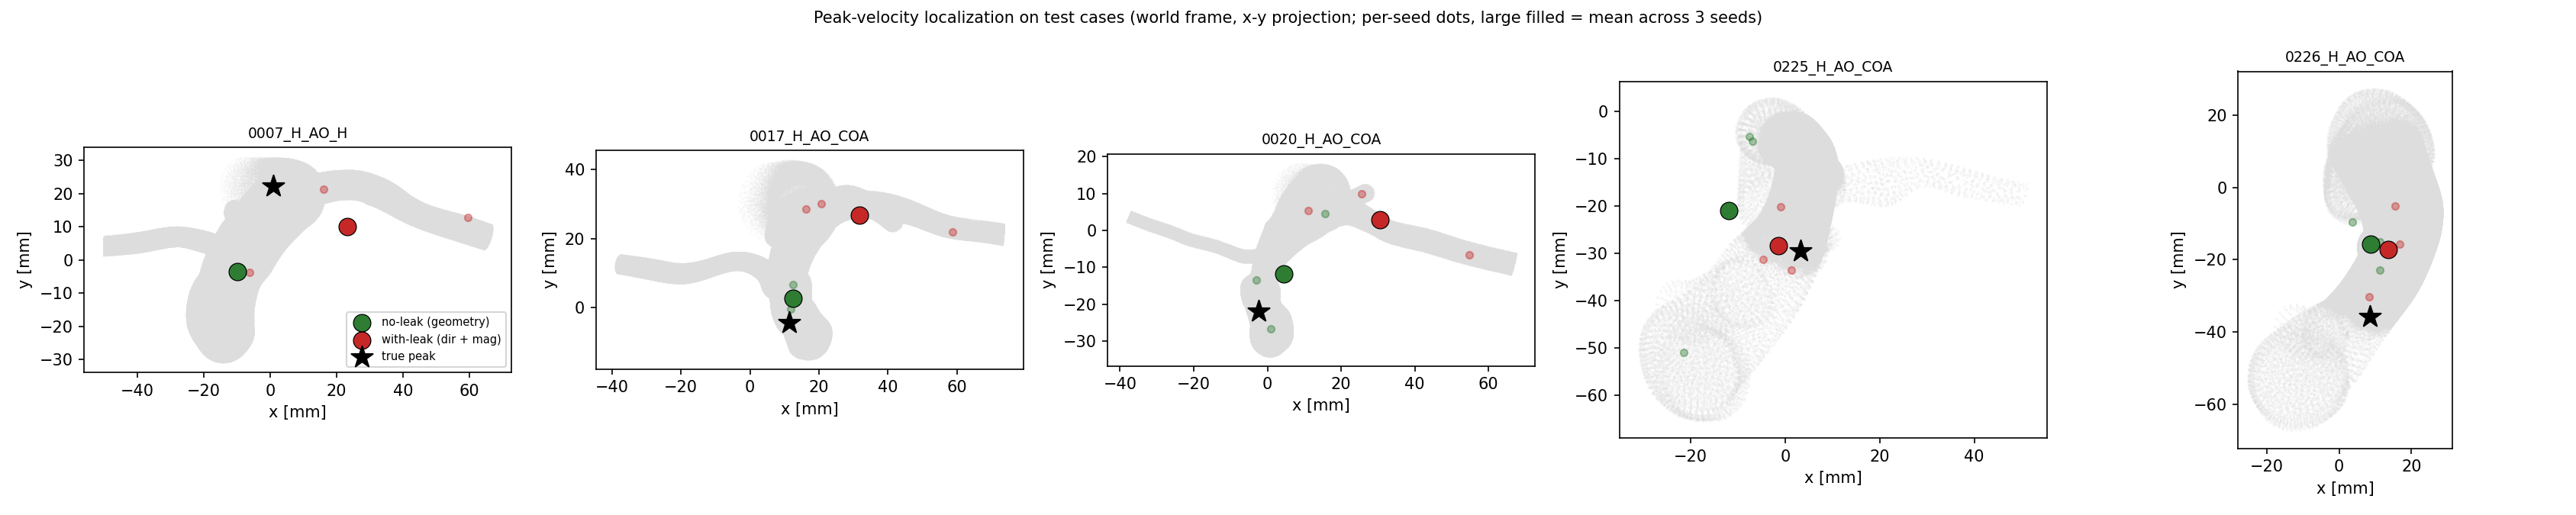
\includegraphics[width=0.9\linewidth]{fig4_peak_world_map.png}
\caption{\textbf{Predicted peak-magnitude positions overlaid on the
test-case 3-D meshes.} True peak (green star) versus per-(variant,
seed) predicted peak (coloured markers). The two FSI cases
(\texttt{0225}, \texttt{0226}) drive the peak-localisation
statistic-dependence discussed in
\Cref{sec:peakloc}.}
\label{fig:fig4}
\end{figure}

\end{document}
